\newpage
\section{Auswertung}
Für die Auswertung haben wir haben zwei von den vorgestellten Gewichtsmatrizen untersucht. Wir haben uns für die Gewichtsmatrizen 'AddMul' und 'Special' entschieden. Um reproduzierbare Ergebnisse liefern zu können, haben wir aus der 'main.m' zwei Dateien abgeleitet in denen die Konfigurationen der nachfolgenden Bilder hinterlegt sind. Die beiden Dateien heißen 'SettingFileAddMul.m' und 'SettingFileSpecial.m'. Beide Systeme wurde empirisch eingestellt und es wurde versucht ab einem Rauschen von 50\% keine vernünftigen Ergebnisse mehr zu liefern. Außerdem wurden die Bias-Werte und Threshold-Werte voreingestellt.

Als nächstes soll für ein Beispiel besprochen werden, wie die Grafiken zu lesen sind. Dafür benutzen wir die Abbildungen \ref{AddMul_H_40_1} und \ref{AddMul_H_40_2} heran. Untersucht wurde die AddMul-Gewichtsmatrix mit horizontalen Balken. Der Rauschwert ist auf 40\% eingestellt. Die Farbe der eingezeichneten Punkte gibt an, ob das jeweilige Merkmal richtig detektiert wurde oder nicht. In Abbildung \ref{AddMul_H_40_1} sehen wir das Ergebnis der ersten Neuronen Ebene. In der Sigmoid-Grafik sind 25 grüne Punkte eingezeichnet. Es sind also alle Merkmale richtig detektiert worden. An dieser Stelle werden die addierten Werte der einzelnen Pixel auf eine Sigmoid-Funktion gegeben und grafisch ausgewertet.

In Abbildung \ref{AddMul_H_40_2} ist die zweite Neuronen-Ebene dargestellt. In jeder Grafik ist jeweils ein Punkt eingezeichnet. In der Grafik der 'h-Balken Detektion' ist ein grüner Punkt eingezeichnet, d.h. es wurde ein 'h-Balken' detektiert. In der Grafik der 'v-Balken Detektion' ist ein roter Punkt eingezeichnet, d.h. es wurde kein 'v-Balken' detektiert. Die letzte Grafik der zweiten Neuronen Ebene ist die 'Fehler Detektion'. In diesem Fall ist der Punkt grün, also wurde keinen Fehler detektiert. Die 'Fehler Detektion' soll angeben, wenn der voreingestellte Rauschwert überschritten wurde. Es ist zu beachten, dass die Werte aus der ersten Ebene nicht mit der Sigmoid-Funktion bearbeitet wurden, sondern lediglich mit einer linearen Aktivierungsfunktion mit dem Anstieg 1, d.h. die addierten Werte der Pixel pro Merkmal werden direkt weitergereicht.  

\newpage
\subsection{AddMul Gewichtsmatrix}
\subsubsection{H-Balken}
\begin{figure}[hbt]
	\centering
	\begin{minipage}[c]{\textwidth}
       	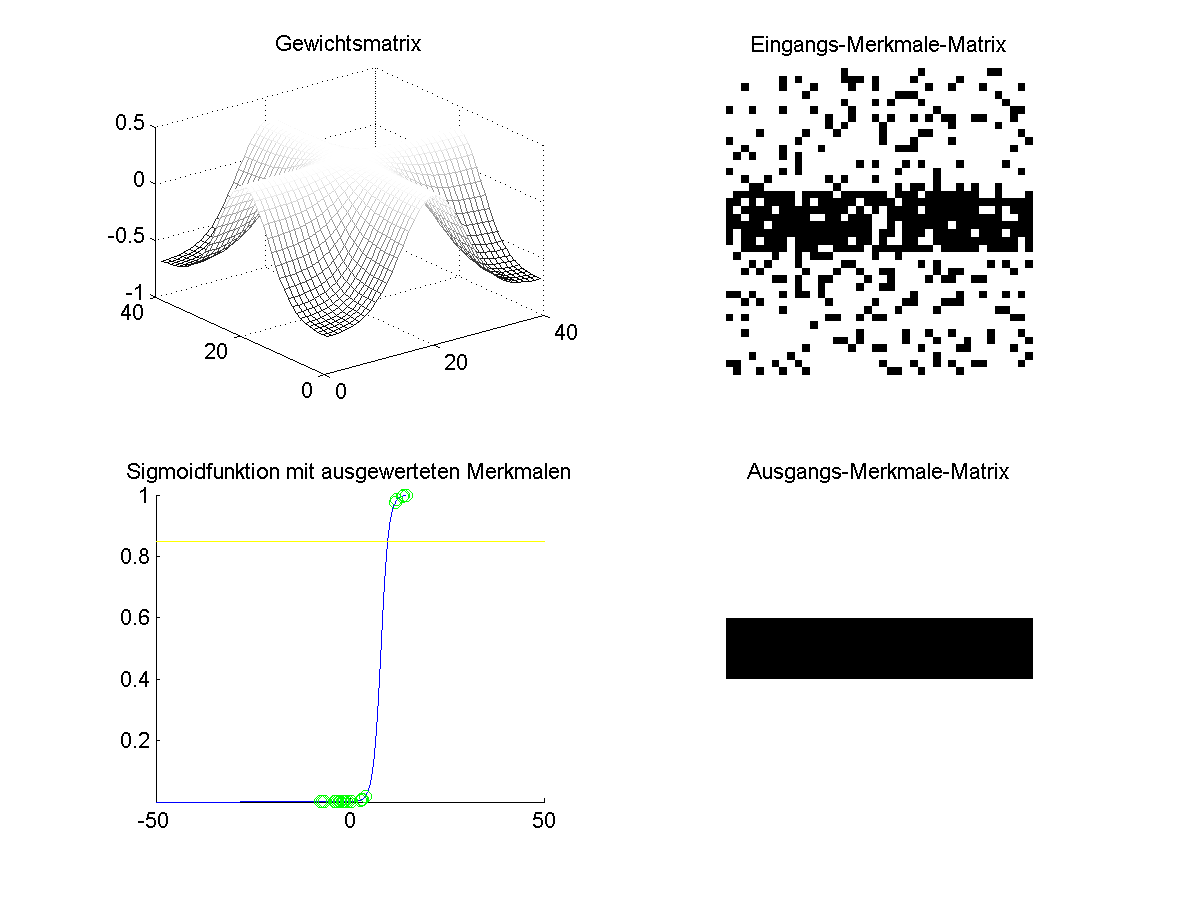
\includegraphics[trim=70 211 42 222, clip, width=0.9\textwidth]{./Bilder/Auswertung/Endergebnis/TypeAddMul_Rauschen40_H_Line_Layer1}
		\caption{AddMul, H-Balken, 40\% Rauschen, 1. Neuronen Ebene}
		\label{AddMul_H_40_1}
		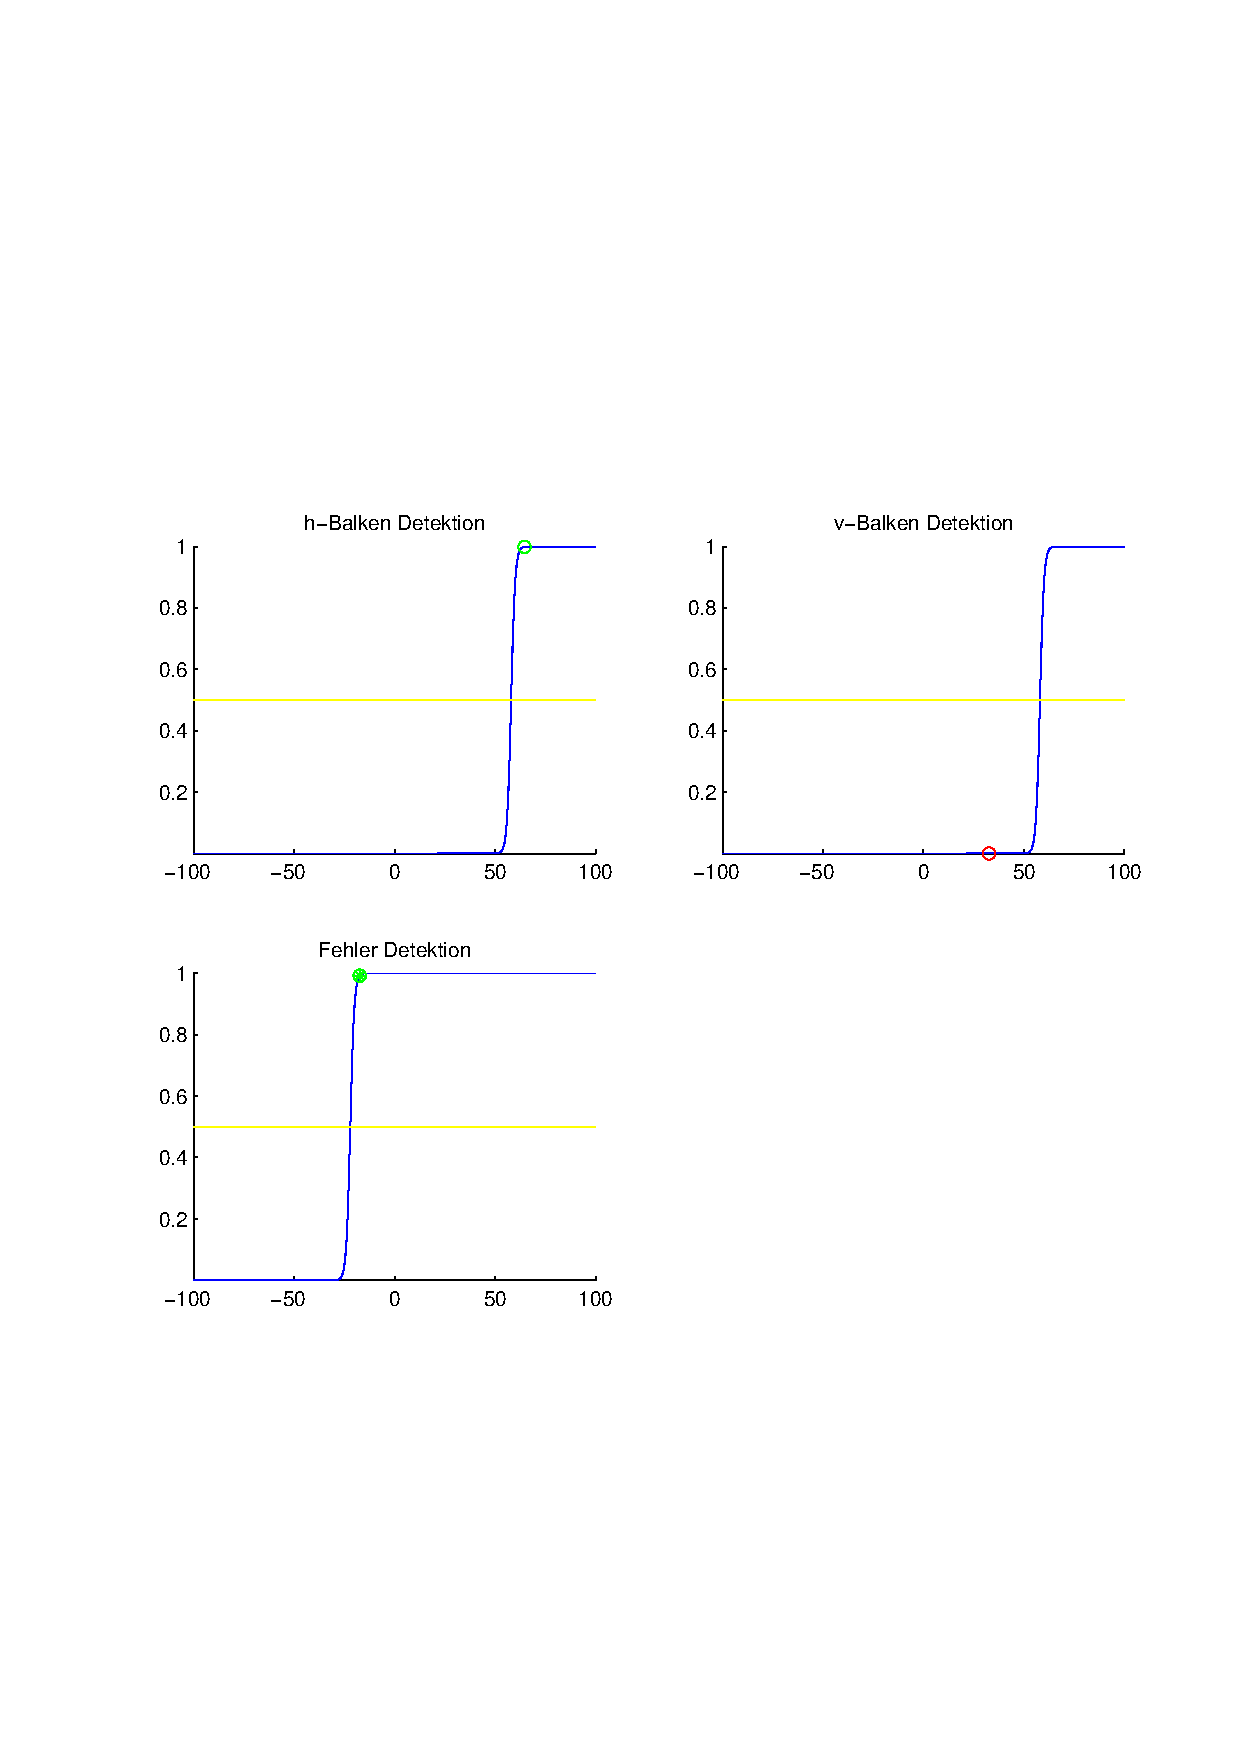
\includegraphics[trim=70 211 42 222, clip, width=0.9\textwidth]{./Bilder/Auswertung/Endergebnis/TypeAddMul_Rauschen40_H_Line_Layer2}
		\caption{AddMul, H-Balken, 40\% Rauschen, 2. Neuronen Ebene}
		\label{AddMul_H_40_2}
	\end{minipage}
\end{figure}

\begin{figure}[hbt]
	\begin{minipage}{0.8 \textwidth}
		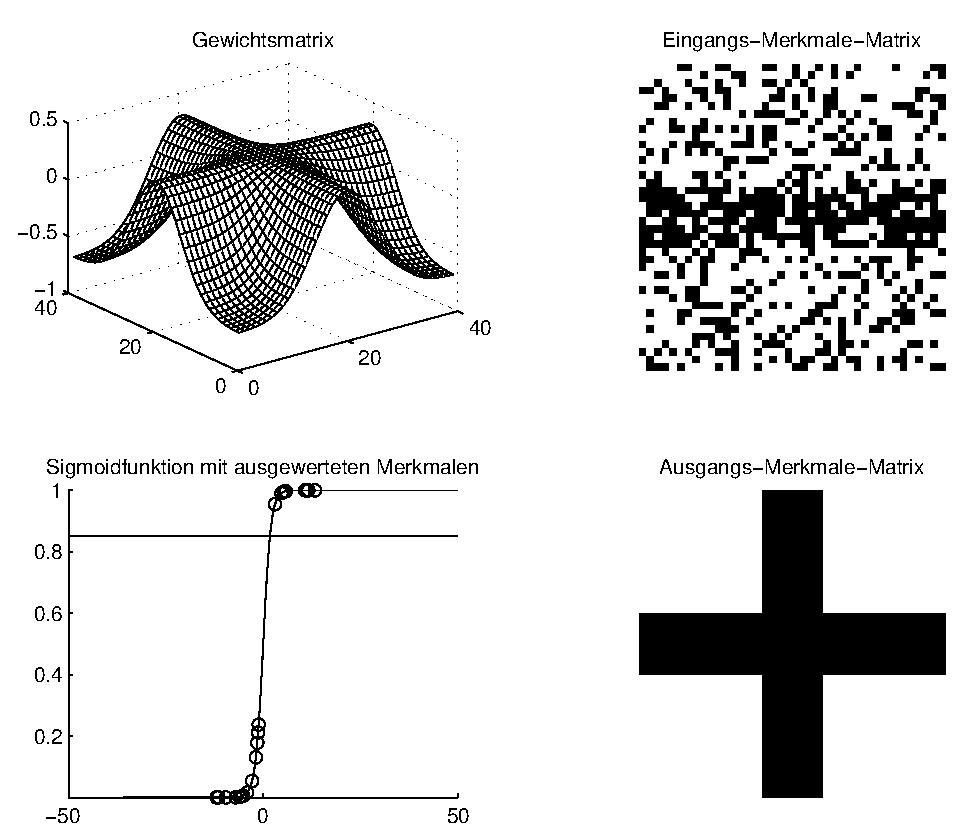
\includegraphics[width=\textwidth]{./Bilder/Auswertung/Endergebnis/TypeAddMul_Rauschen60_H_Line_Layer1}
		\caption{AddMul, H-Balken, 60\% Rauschen, 1. Neuronen Ebene}
		\label{AddMul_H_60_1}
	\end{minipage}
	\vfill
	\begin{minipage}{0.8 \textwidth}
		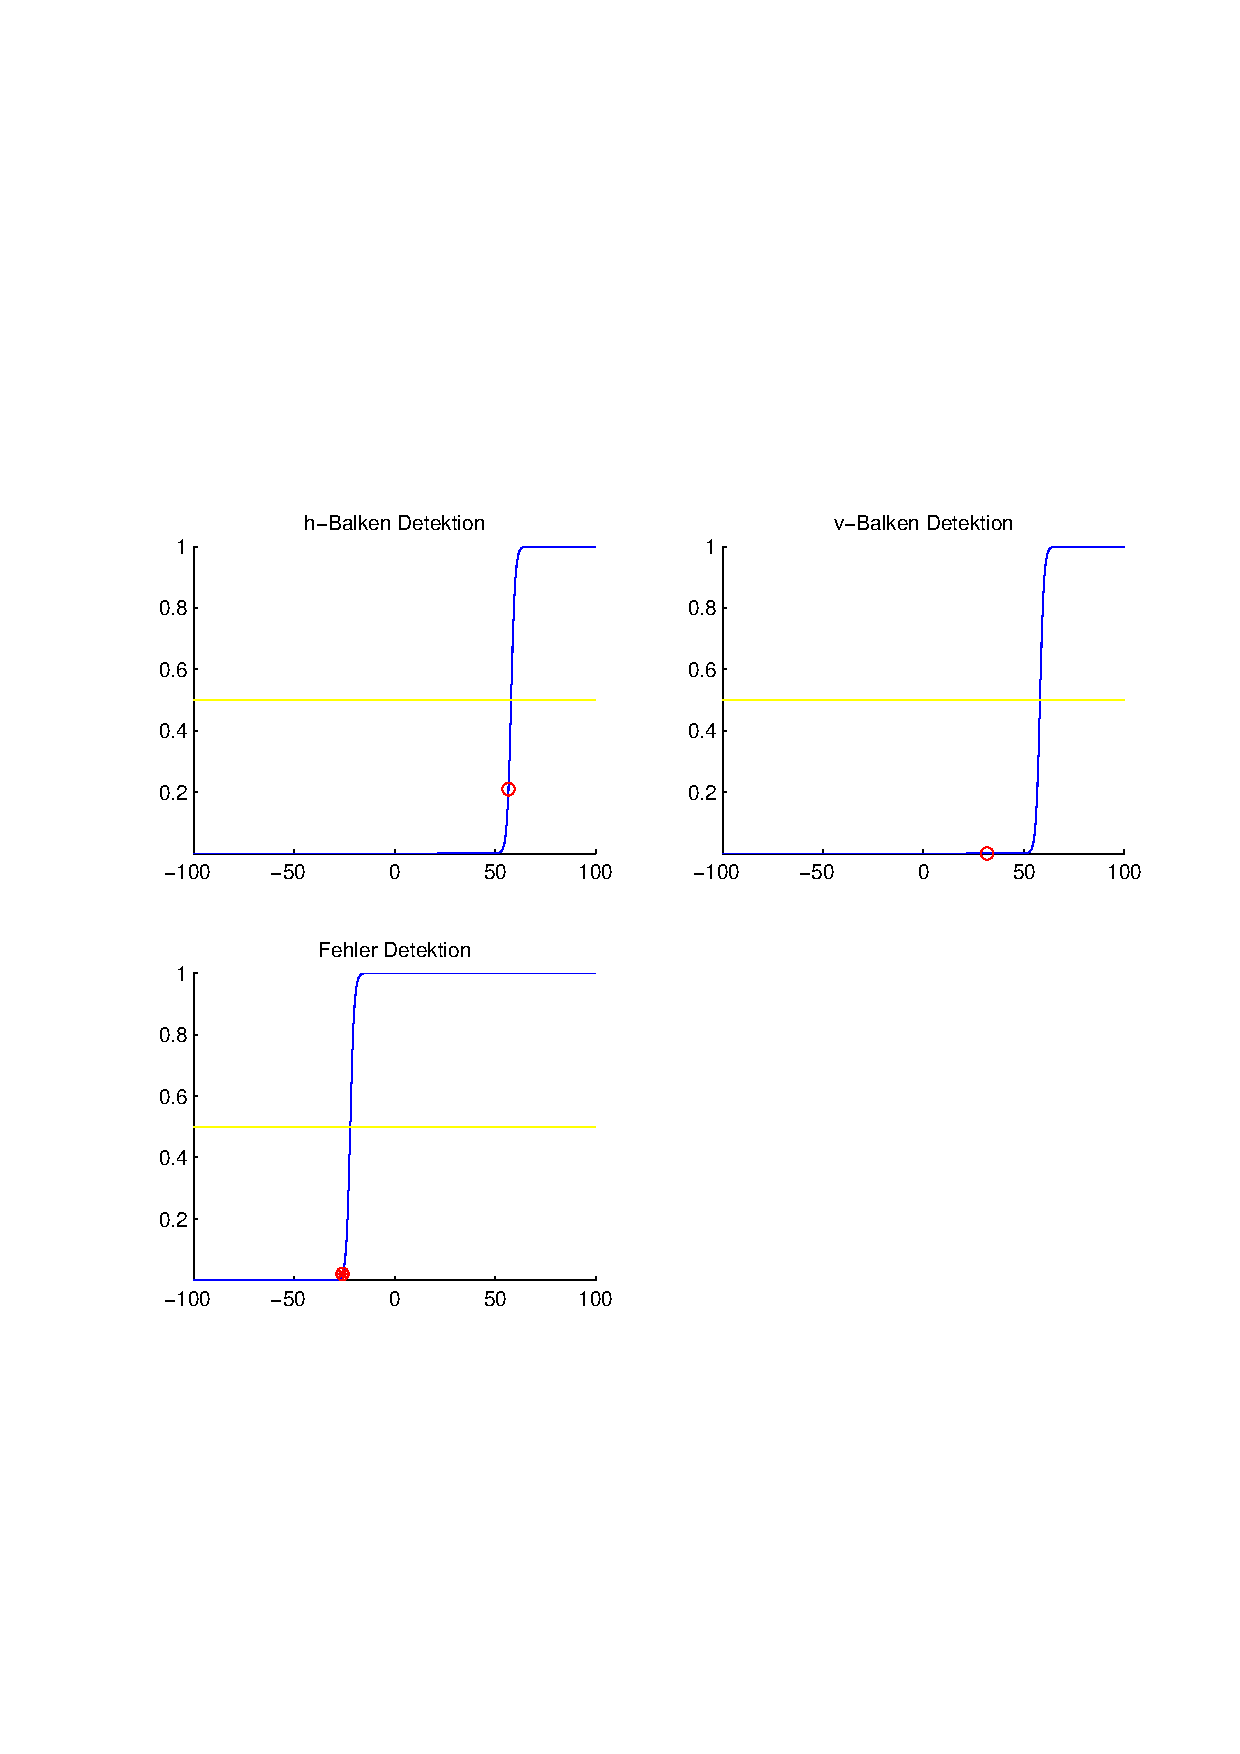
\includegraphics[width=\textwidth]{./Bilder/Auswertung/Endergebnis/TypeAddMul_Rauschen60_H_Line_Layer2}
		\caption{AddMul, H-Balken, 60\% Rauschen, 2. Neuronen Ebene}
		\label{AddMul_H_60_2}
	\end{minipage}
\end{figure}

\begin{figure}[hbt]
	\begin{minipage}{0.8 \textwidth}
		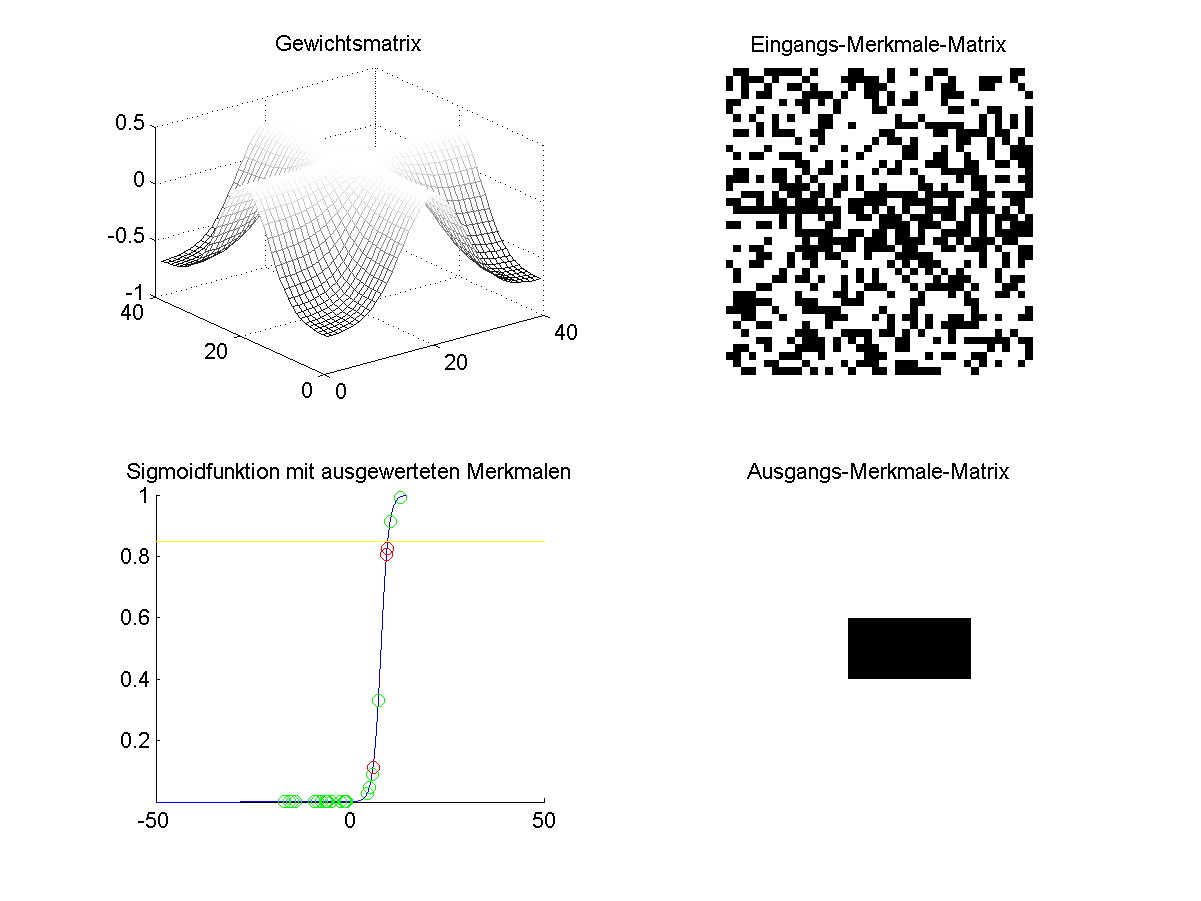
\includegraphics[width=\textwidth]{./Bilder/Auswertung/Endergebnis/TypeAddMul_Rauschen80_H_Line_Layer1}
		\caption{AddMul, H-Balken, 80\% Rauschen, 1. Neuronen Ebene}
		\label{AddMul_H_80_1}
	\end{minipage}
	\vfill
	\begin{minipage}{0.8 \textwidth}
		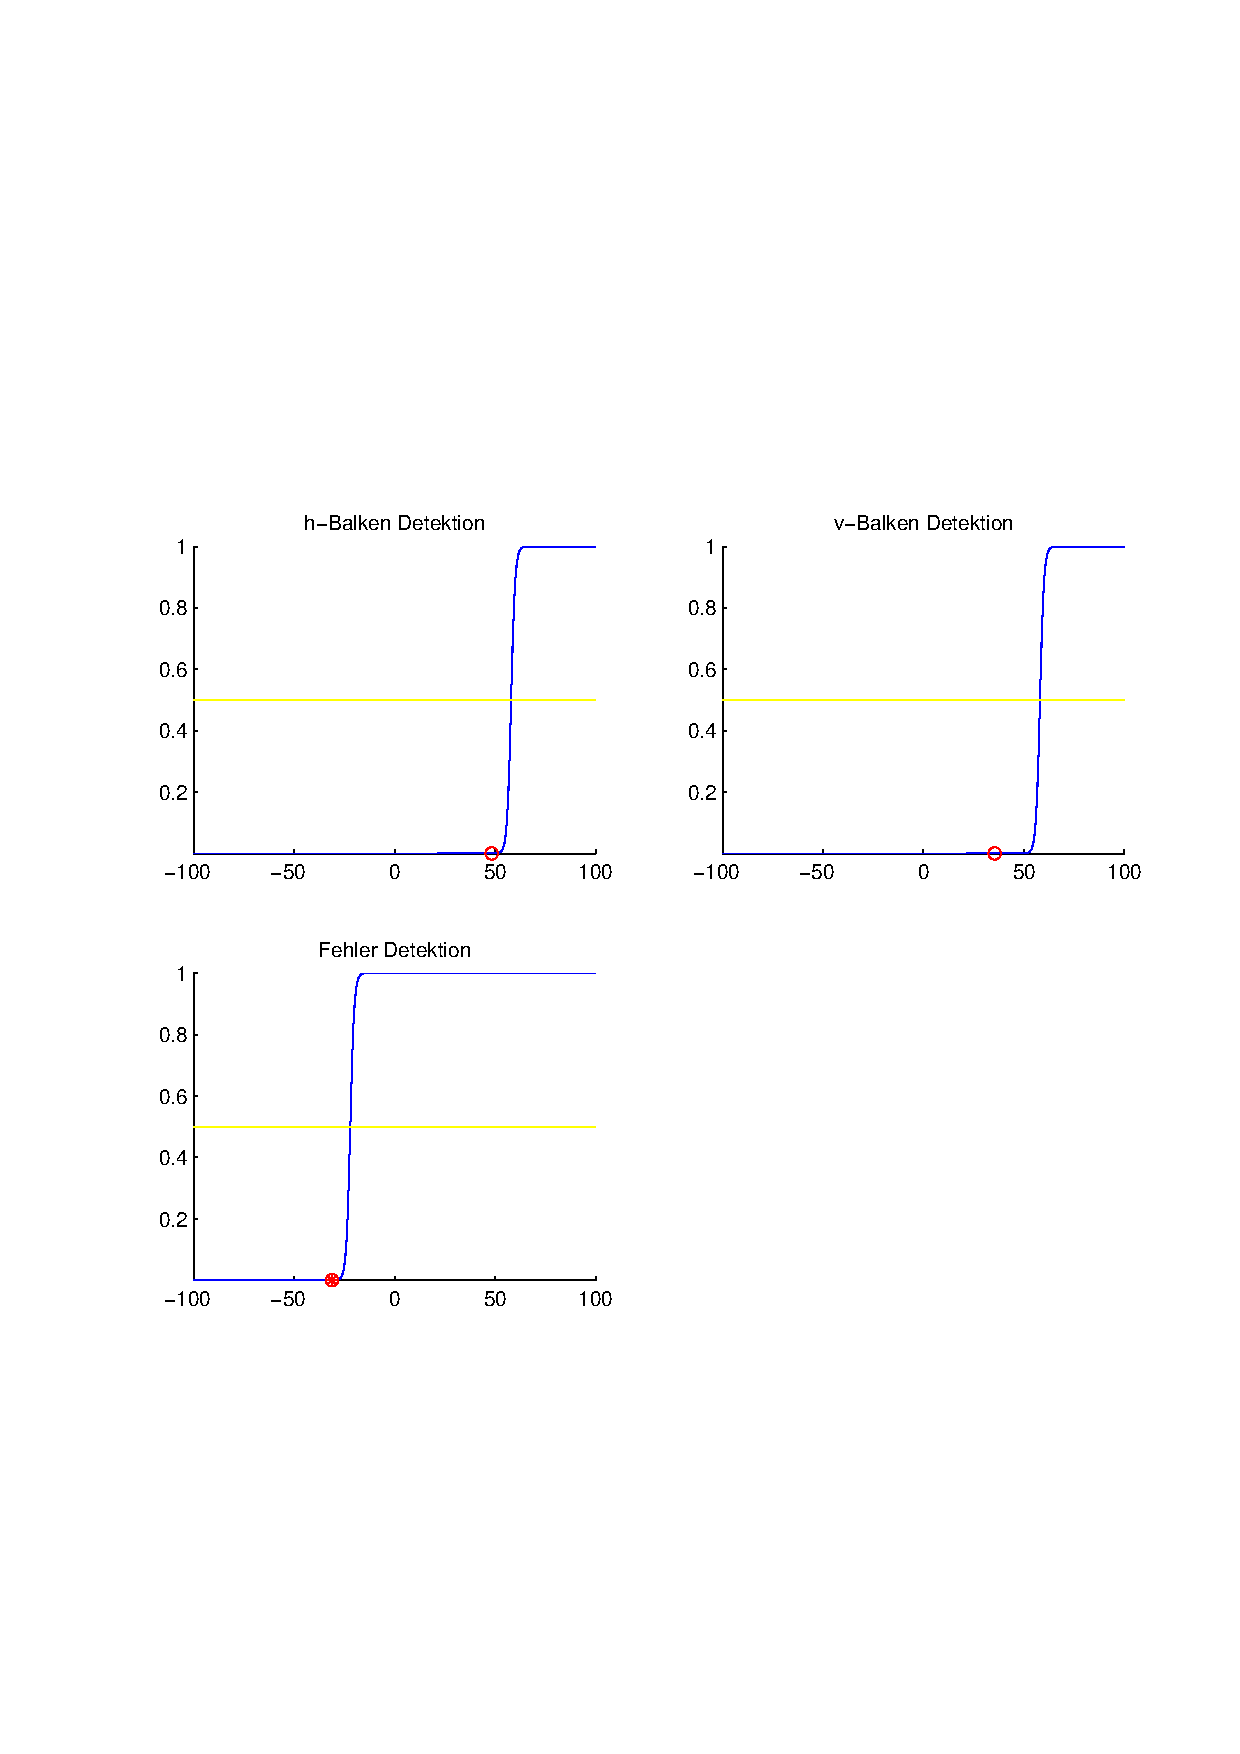
\includegraphics[width=\textwidth]{./Bilder/Auswertung/Endergebnis/TypeAddMul_Rauschen80_H_Line_Layer2}
		\caption{AddMul, H-Balken, 80\% Rauschen, 2. Neuronen Ebene}
		\label{AddMul_H_80_2}
	\end{minipage}
\end{figure}
\clearpage

\subsubsection{V-Balken}
\begin{figure}[hbt]
	\begin{minipage}{0.8 \textwidth}
		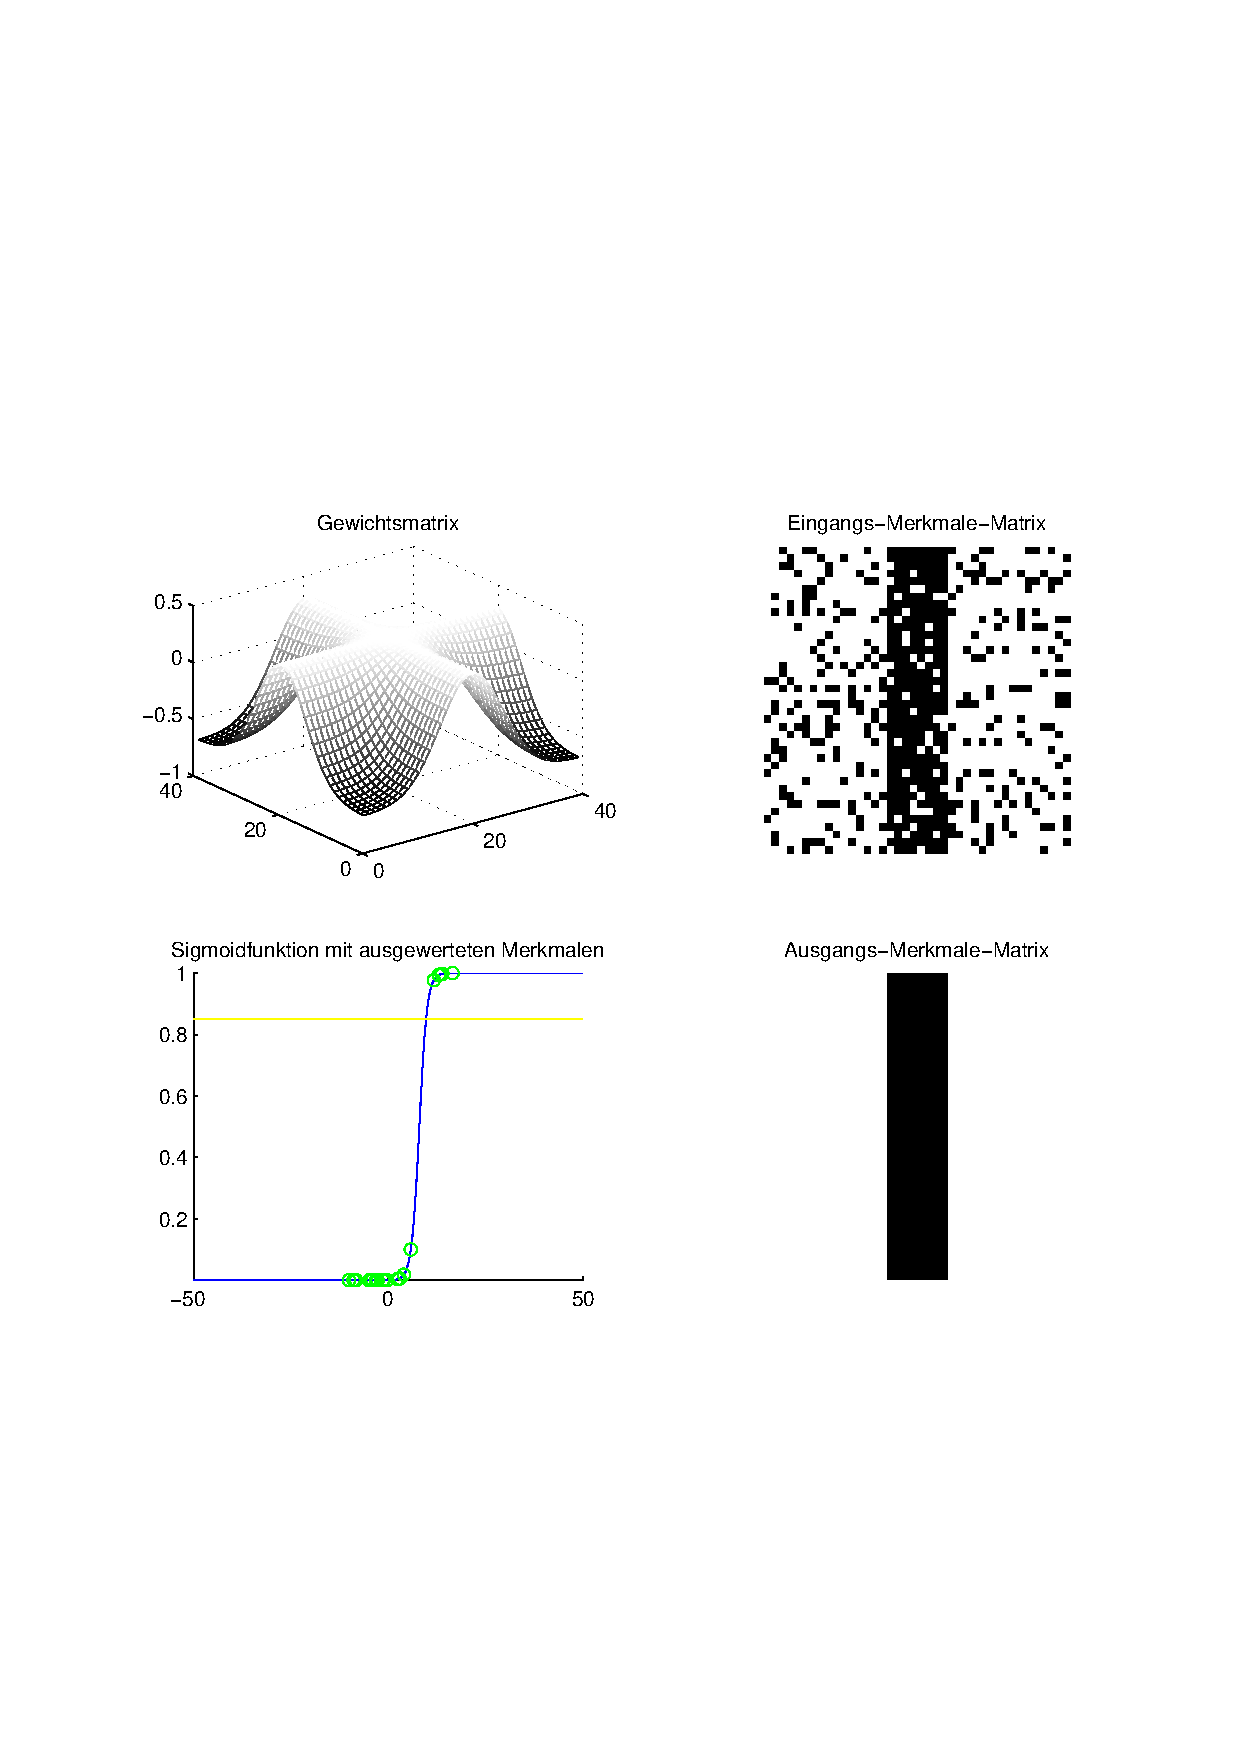
\includegraphics[width=\textwidth]{./Bilder/Auswertung/Endergebnis/TypeAddMul_Rauschen40_V_Line_Layer1}
		\caption{AddMul, V-Balken, 40\% Rauschen, 1. Neuronen Ebene}
		\label{AddMul_V_40_1}
	\end{minipage}
	\vfill
	\begin{minipage}{0.8 \textwidth}
		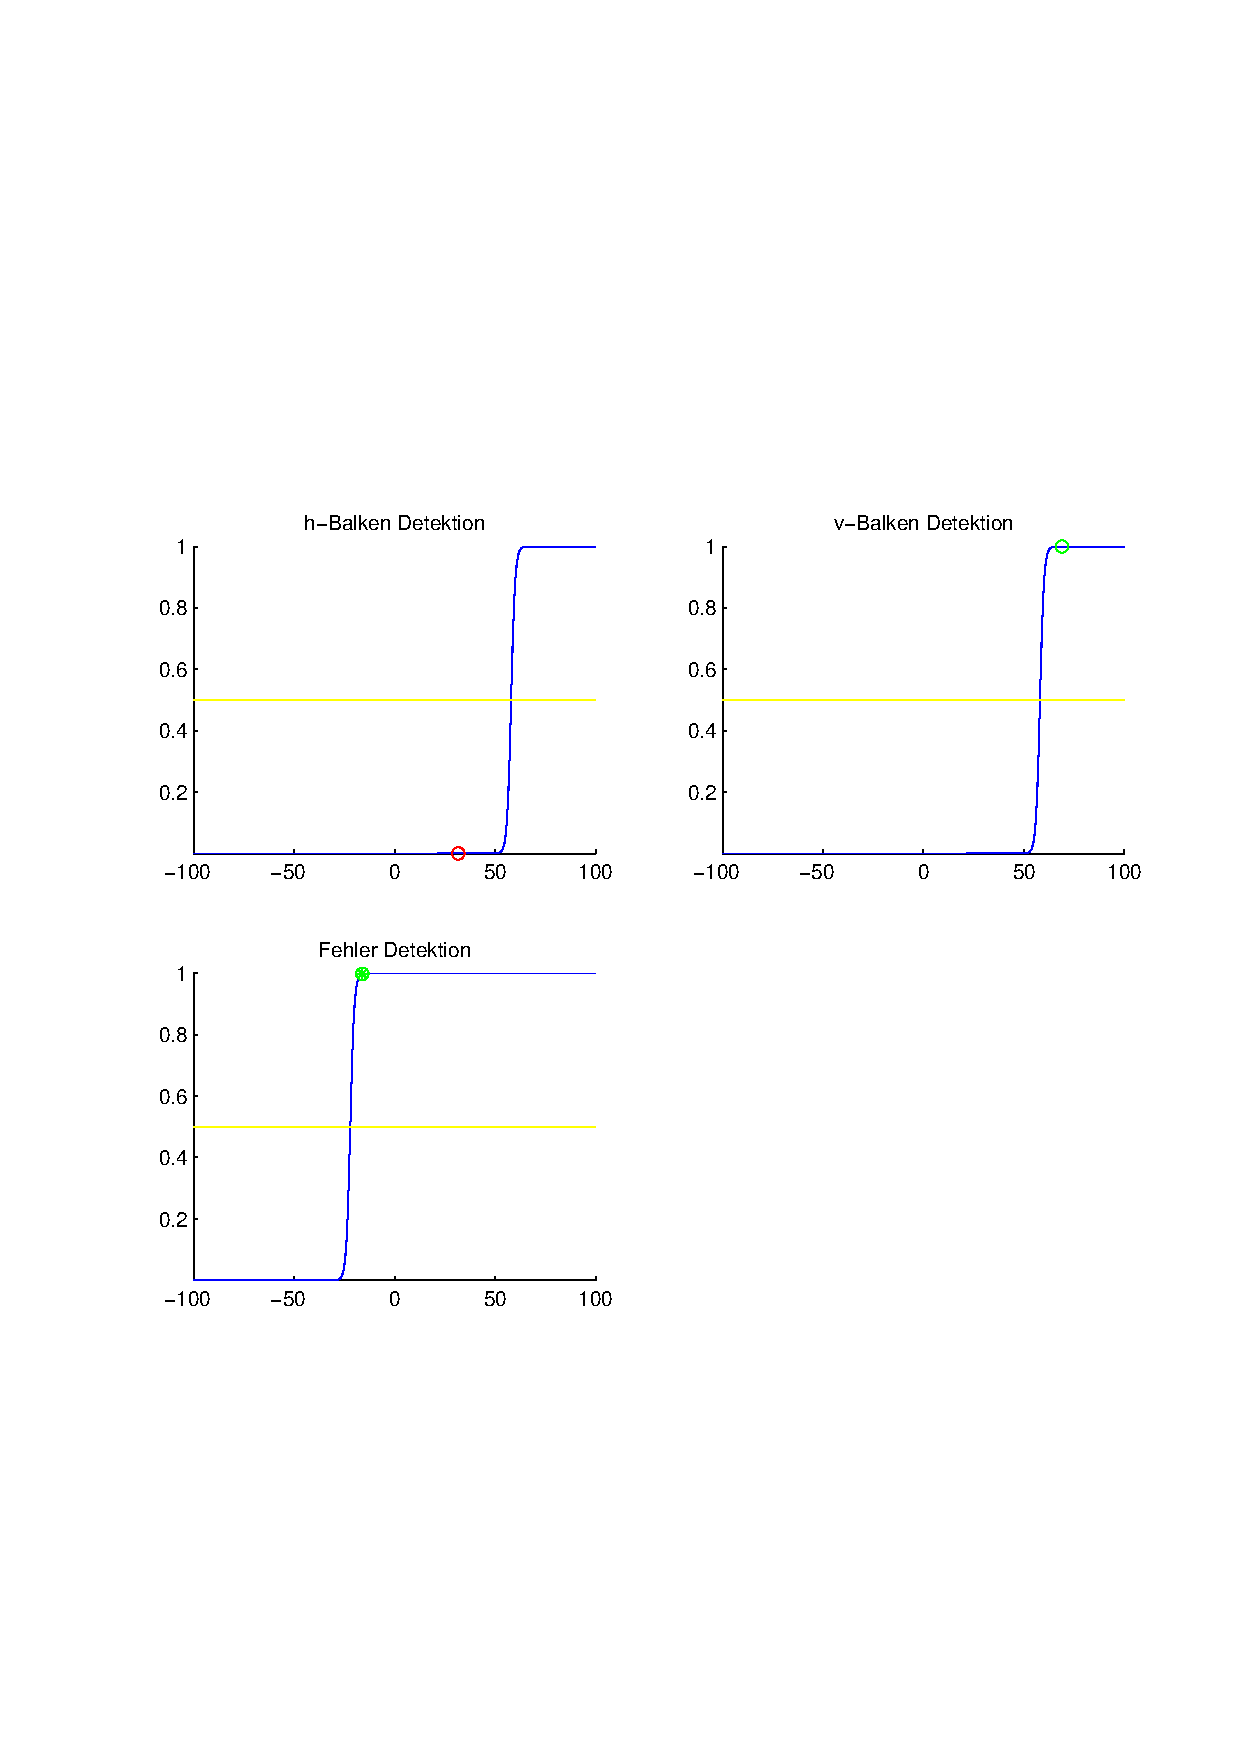
\includegraphics[width=\textwidth]{./Bilder/Auswertung/Endergebnis/TypeAddMul_Rauschen40_V_Line_Layer2}
		\caption{AddMul, V-Balken, 40\% Rauschen, 2. Neuronen Ebene}
		\label{AddMul_V_40_2}
	\end{minipage}
\end{figure}

\begin{figure}[hbt]
	\begin{minipage}{0.8 \textwidth}
		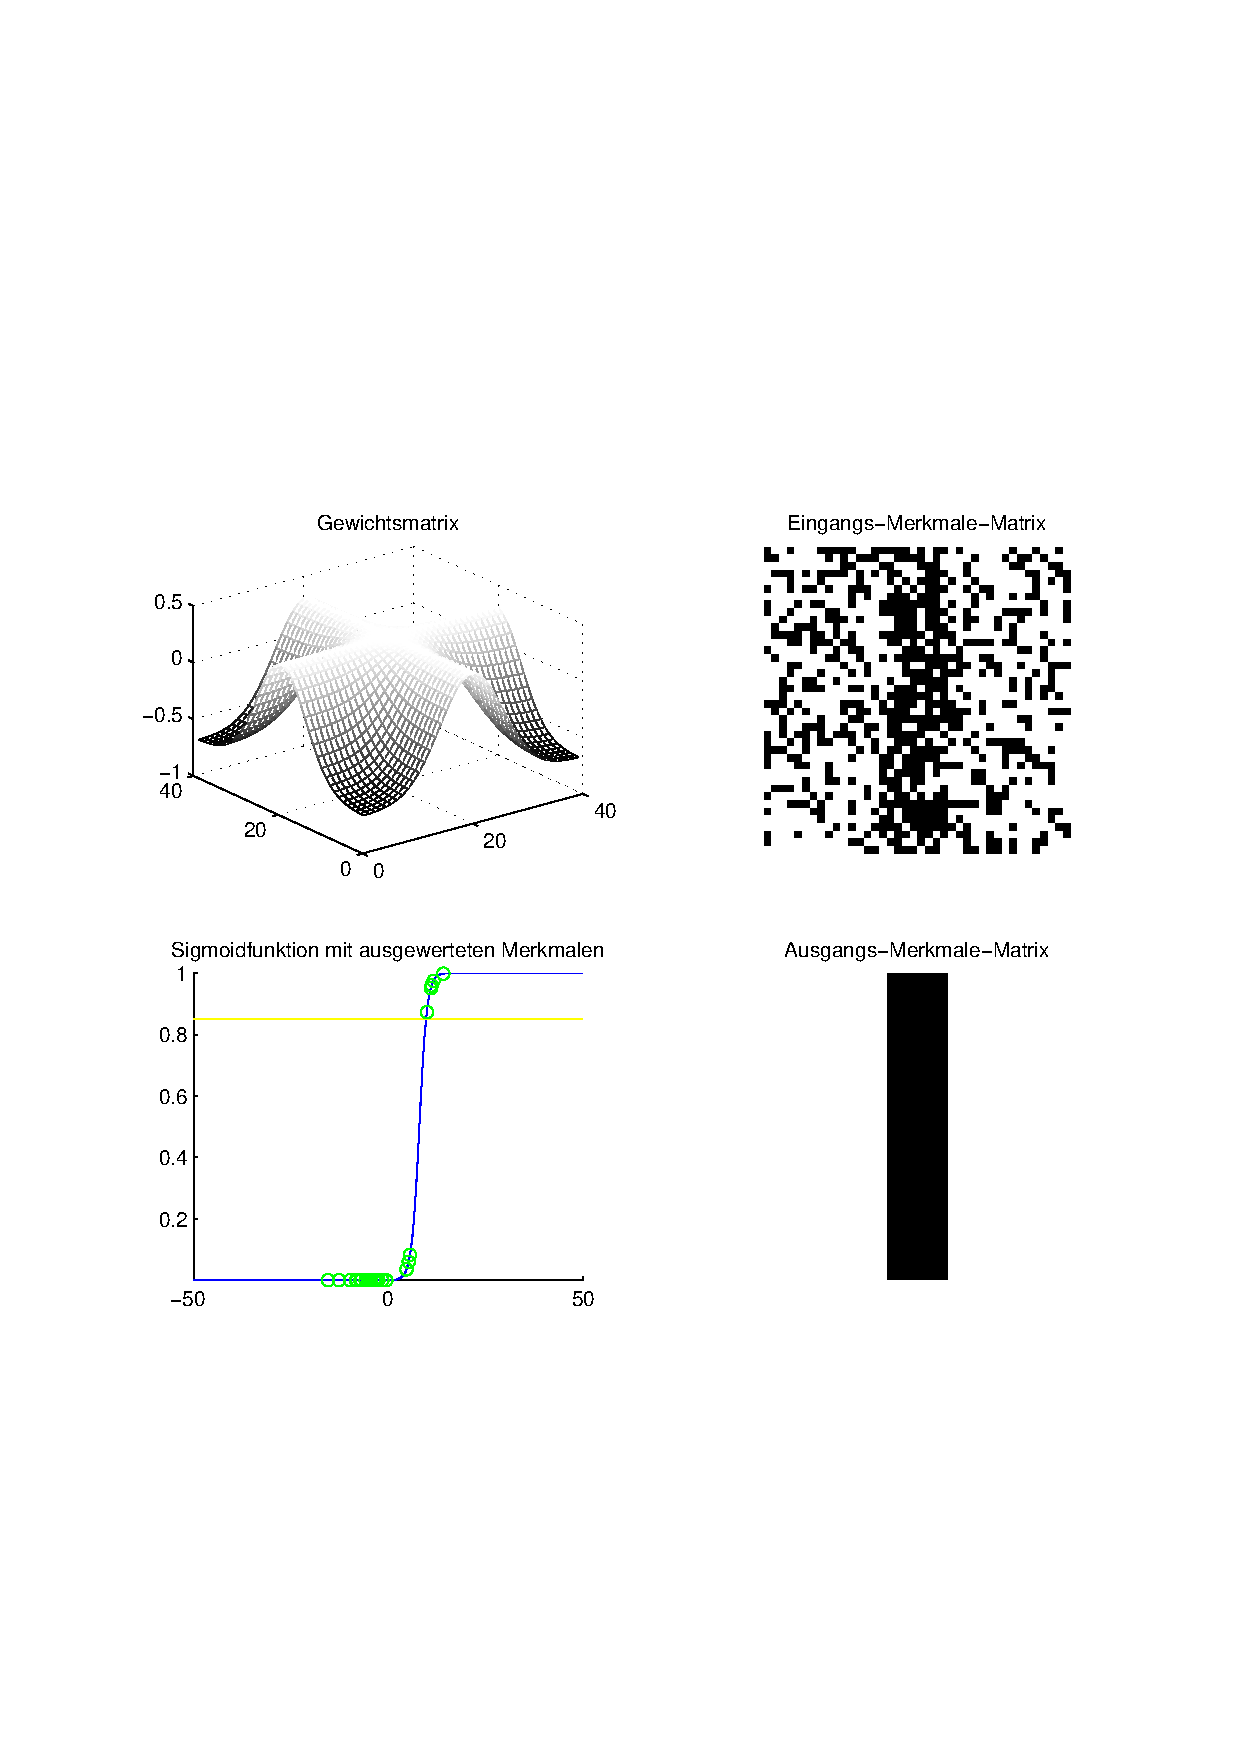
\includegraphics[width=\textwidth]{./Bilder/Auswertung/Endergebnis/TypeAddMul_Rauschen60_V_Line_Layer1}
		\caption{AddMul, V-Balken, 60\% Rauschen, 1. Neuronen Ebene}
		\label{AddMul_V_60_1}
	\end{minipage}
	\vfill
	\begin{minipage}{0.8 \textwidth}
		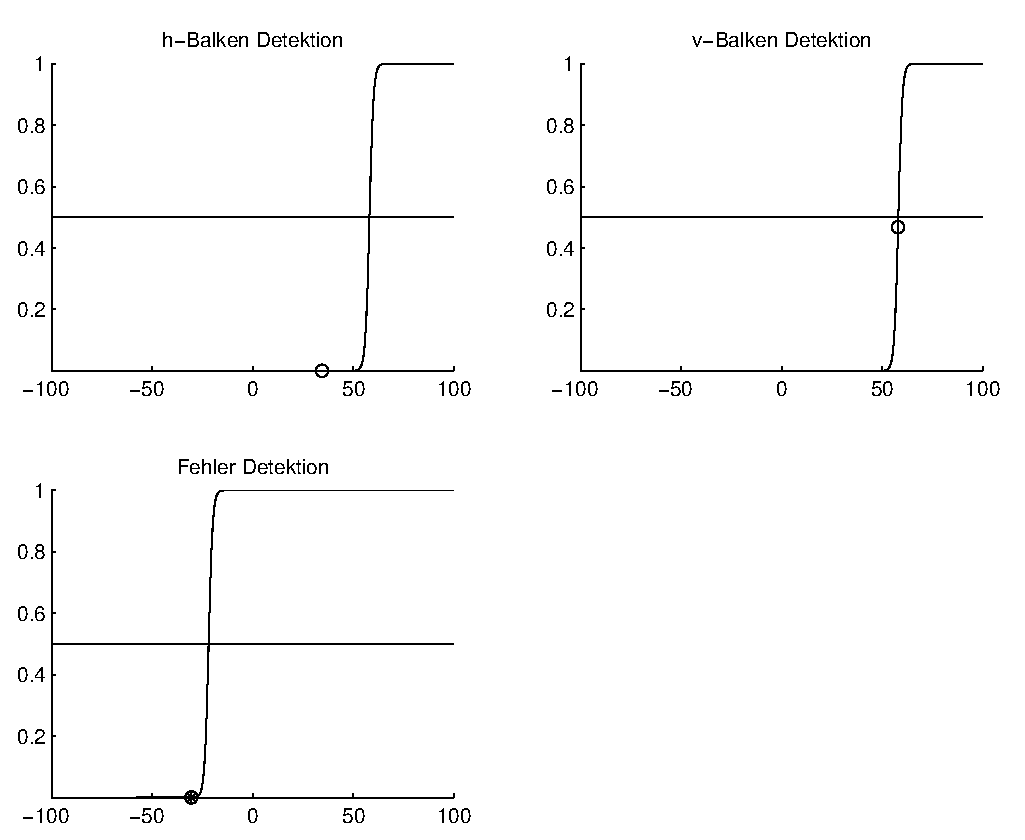
\includegraphics[width=\textwidth]{./Bilder/Auswertung/Endergebnis/TypeAddMul_Rauschen60_V_Line_Layer2}
		\caption{AddMul, V-Balken, 60\% Rauschen, 2. Neuronen Ebene}
		\label{AddMul_V_60_2}
	\end{minipage}
\end{figure}

\begin{figure}[hbt]
	\begin{minipage}{0.8 \textwidth}
		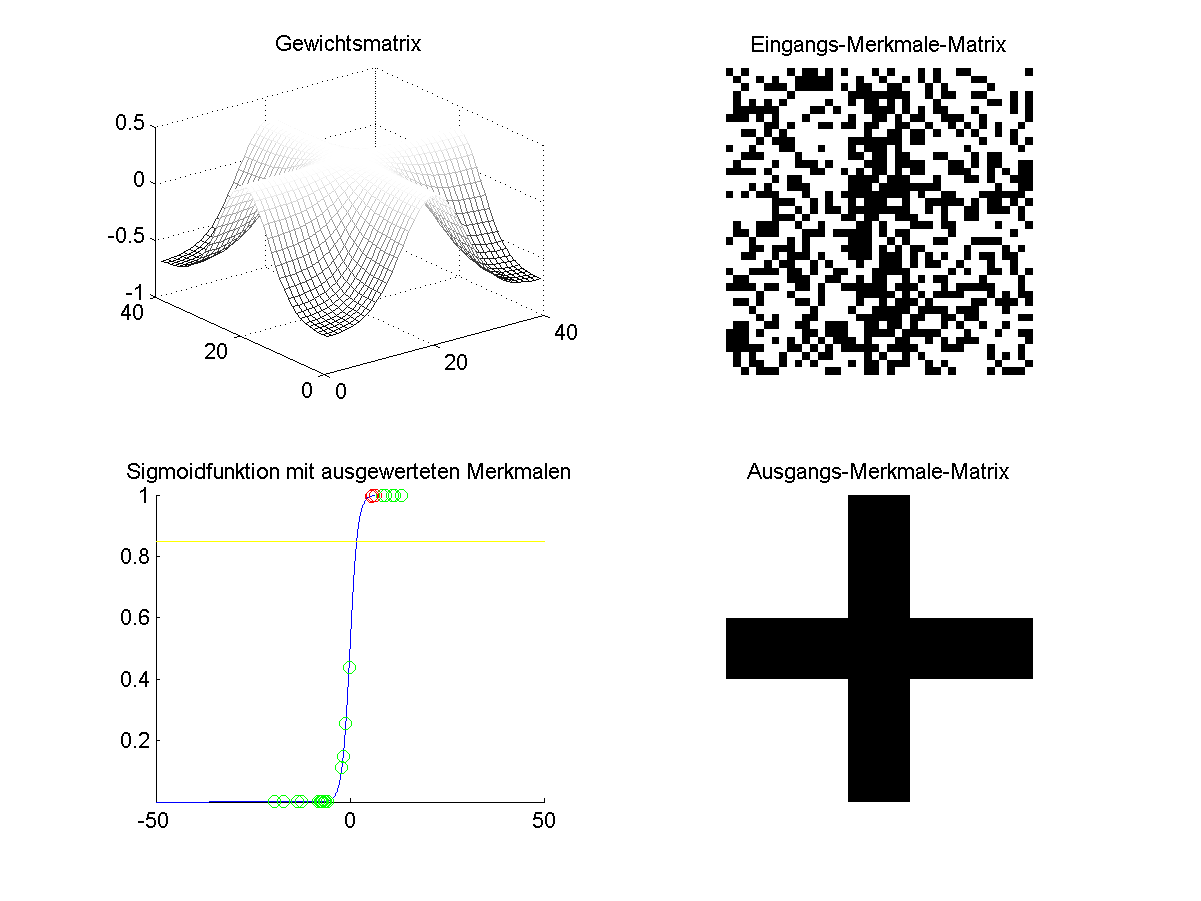
\includegraphics[width=\textwidth]{./Bilder/Auswertung/Endergebnis/TypeAddMul_Rauschen80_V_Line_Layer1}
		\caption{AddMul, V-Balken, 80\% Rauschen, 1. Neuronen Ebene}
		\label{AddMul_V_80_1}
	\end{minipage}
	\vfill
	\begin{minipage}{0.8 \textwidth}
		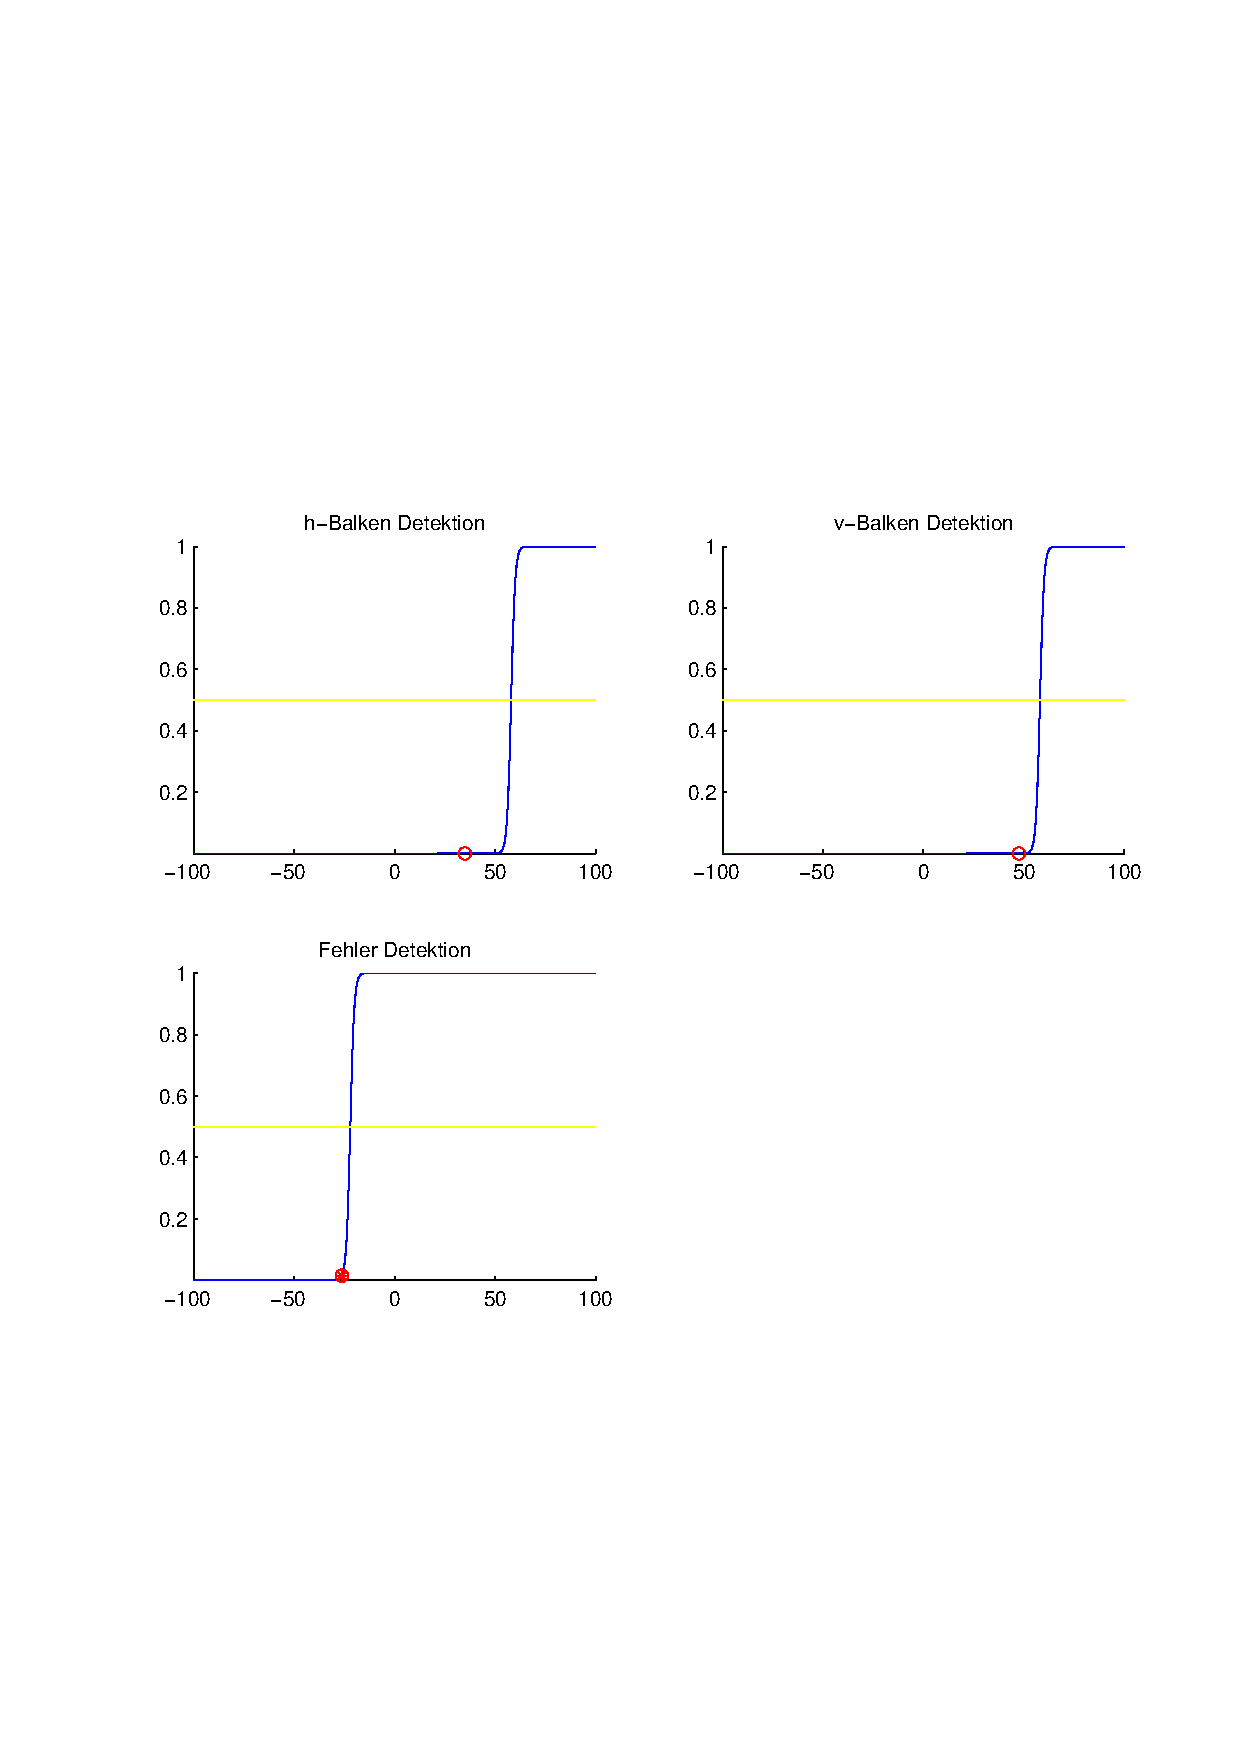
\includegraphics[width=\textwidth]{./Bilder/Auswertung/Endergebnis/TypeAddMul_Rauschen80_V_Line_Layer2}
		\caption{AddMul, V-Balken, 80\% Rauschen, 2. Neuronen Ebene}
		\label{AddMul_V_80_2}
	\end{minipage}
\end{figure}
\clearpage

\subsubsection{Kreuz}
\begin{figure}[hbt]
	\begin{minipage}{0.8 \textwidth}
		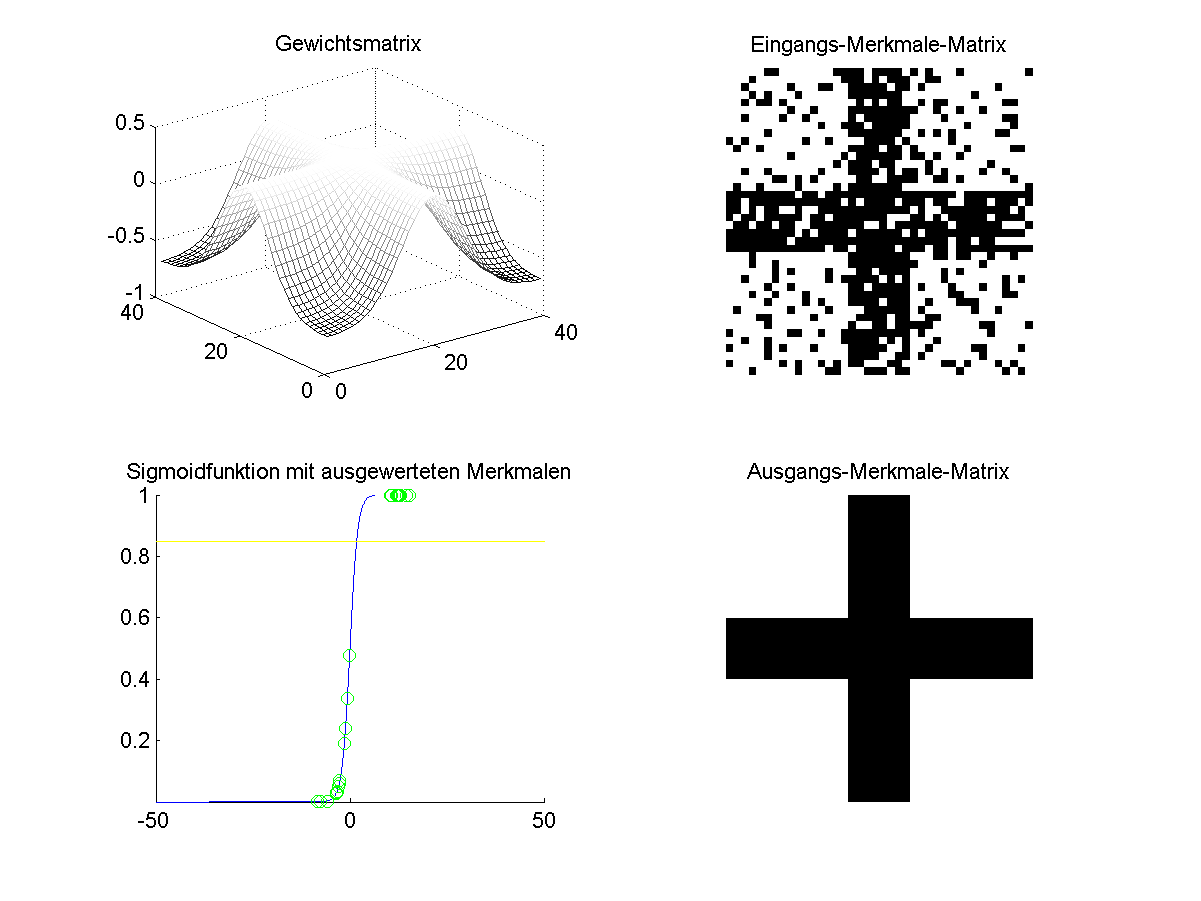
\includegraphics[width=\textwidth]{./Bilder/Auswertung/Endergebnis/TypeAddMul_Rauschen40_Cross_Layer1}
		\caption{AddMul, Kreuz, 40\% Rauschen, 1. Neuronen Ebene}
		\label{AddMul_Kreuz_40_1}
	\end{minipage}
	\vfill
	\begin{minipage}{0.8 \textwidth}
		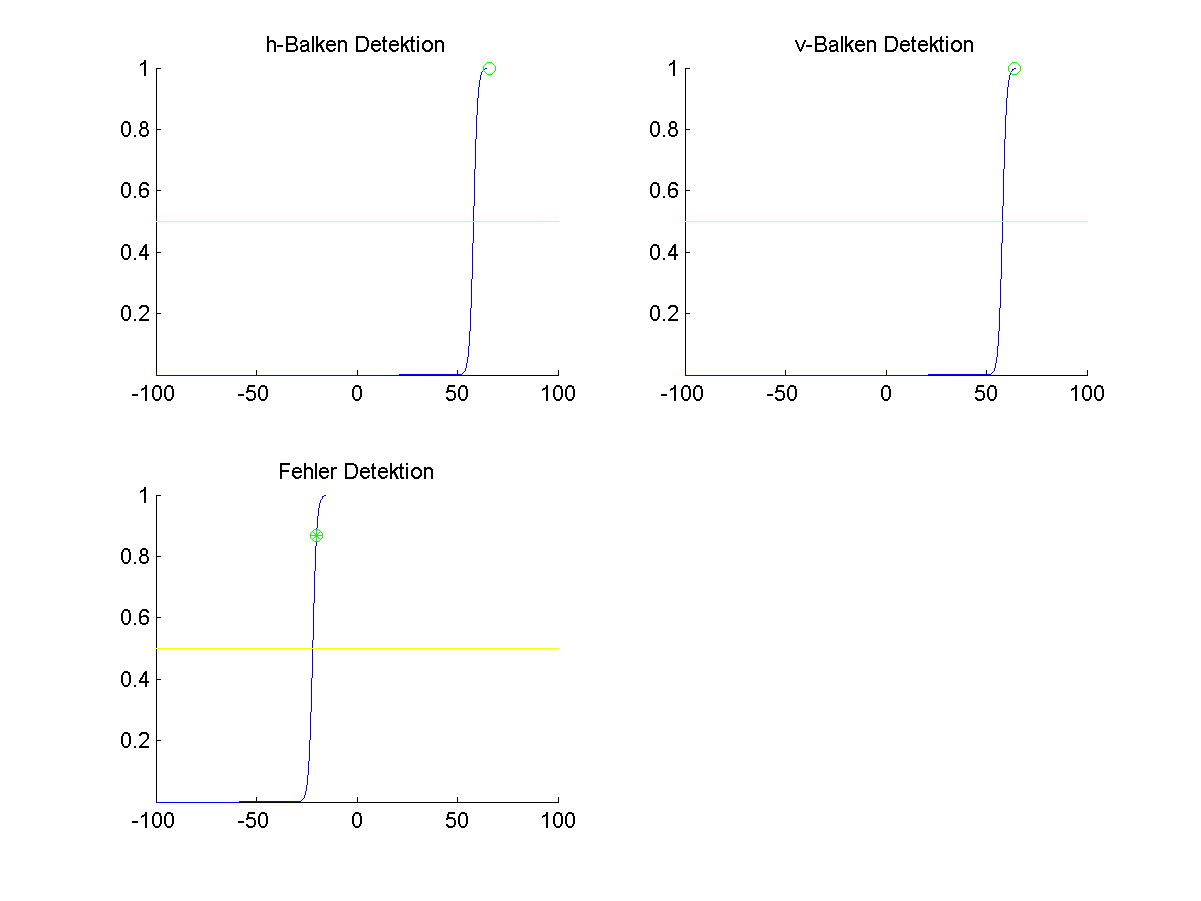
\includegraphics[width=\textwidth]{./Bilder/Auswertung/Endergebnis/TypeAddMul_Rauschen40_Cross_Layer2}
		\caption{AddMul, Kreuz, 40\% Rauschen, 2. Neuronen Ebene}
		\label{AddMul_Kreuz_40_2}
	\end{minipage}
\end{figure}

\begin{figure}[hbt]
	\begin{minipage}{0.8 \textwidth}
		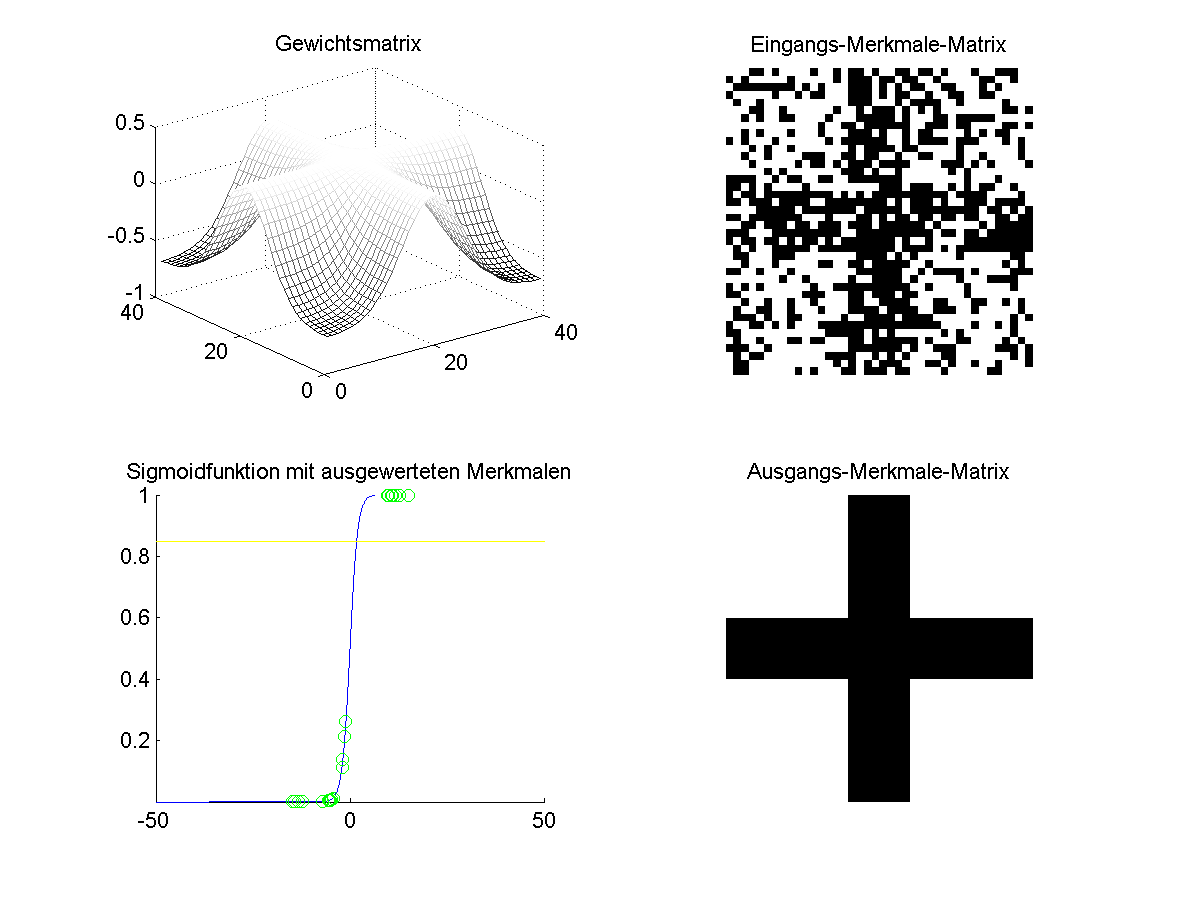
\includegraphics[width=\textwidth]{./Bilder/Auswertung/Endergebnis/TypeAddMul_Rauschen60_Cross_Layer1}
		\caption{AddMul, Kreuz, 60\% Rauschen, 1. Neuronen Ebene}
		\label{AddMul_Kreuz_60_1}
	\end{minipage}
	\vfill
	\begin{minipage}{0.8 \textwidth}
		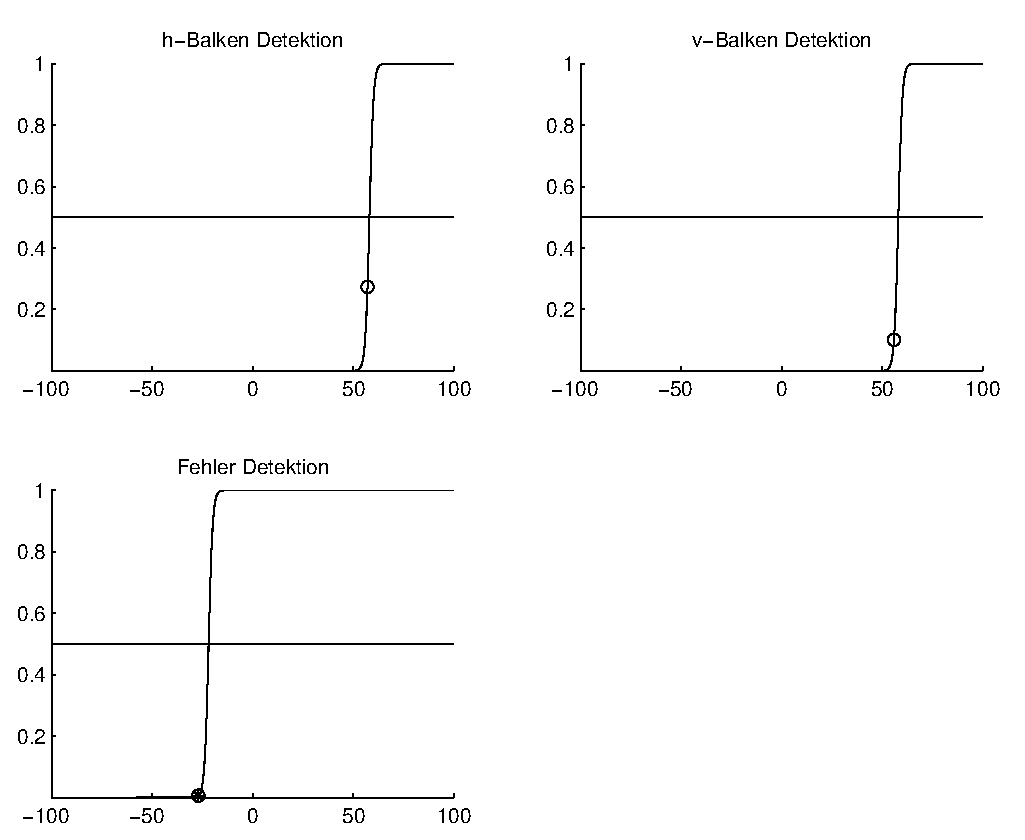
\includegraphics[width=\textwidth]{./Bilder/Auswertung/Endergebnis/TypeAddMul_Rauschen60_Cross_Layer2}
		\caption{AddMul, Kreuz, 60\% Rauschen, 2. Neuronen Ebene}
		\label{AddMul_Kreuz_60_2}
	\end{minipage}
\end{figure}

\begin{figure}[hbt]
	\begin{minipage}{0.8 \textwidth}
		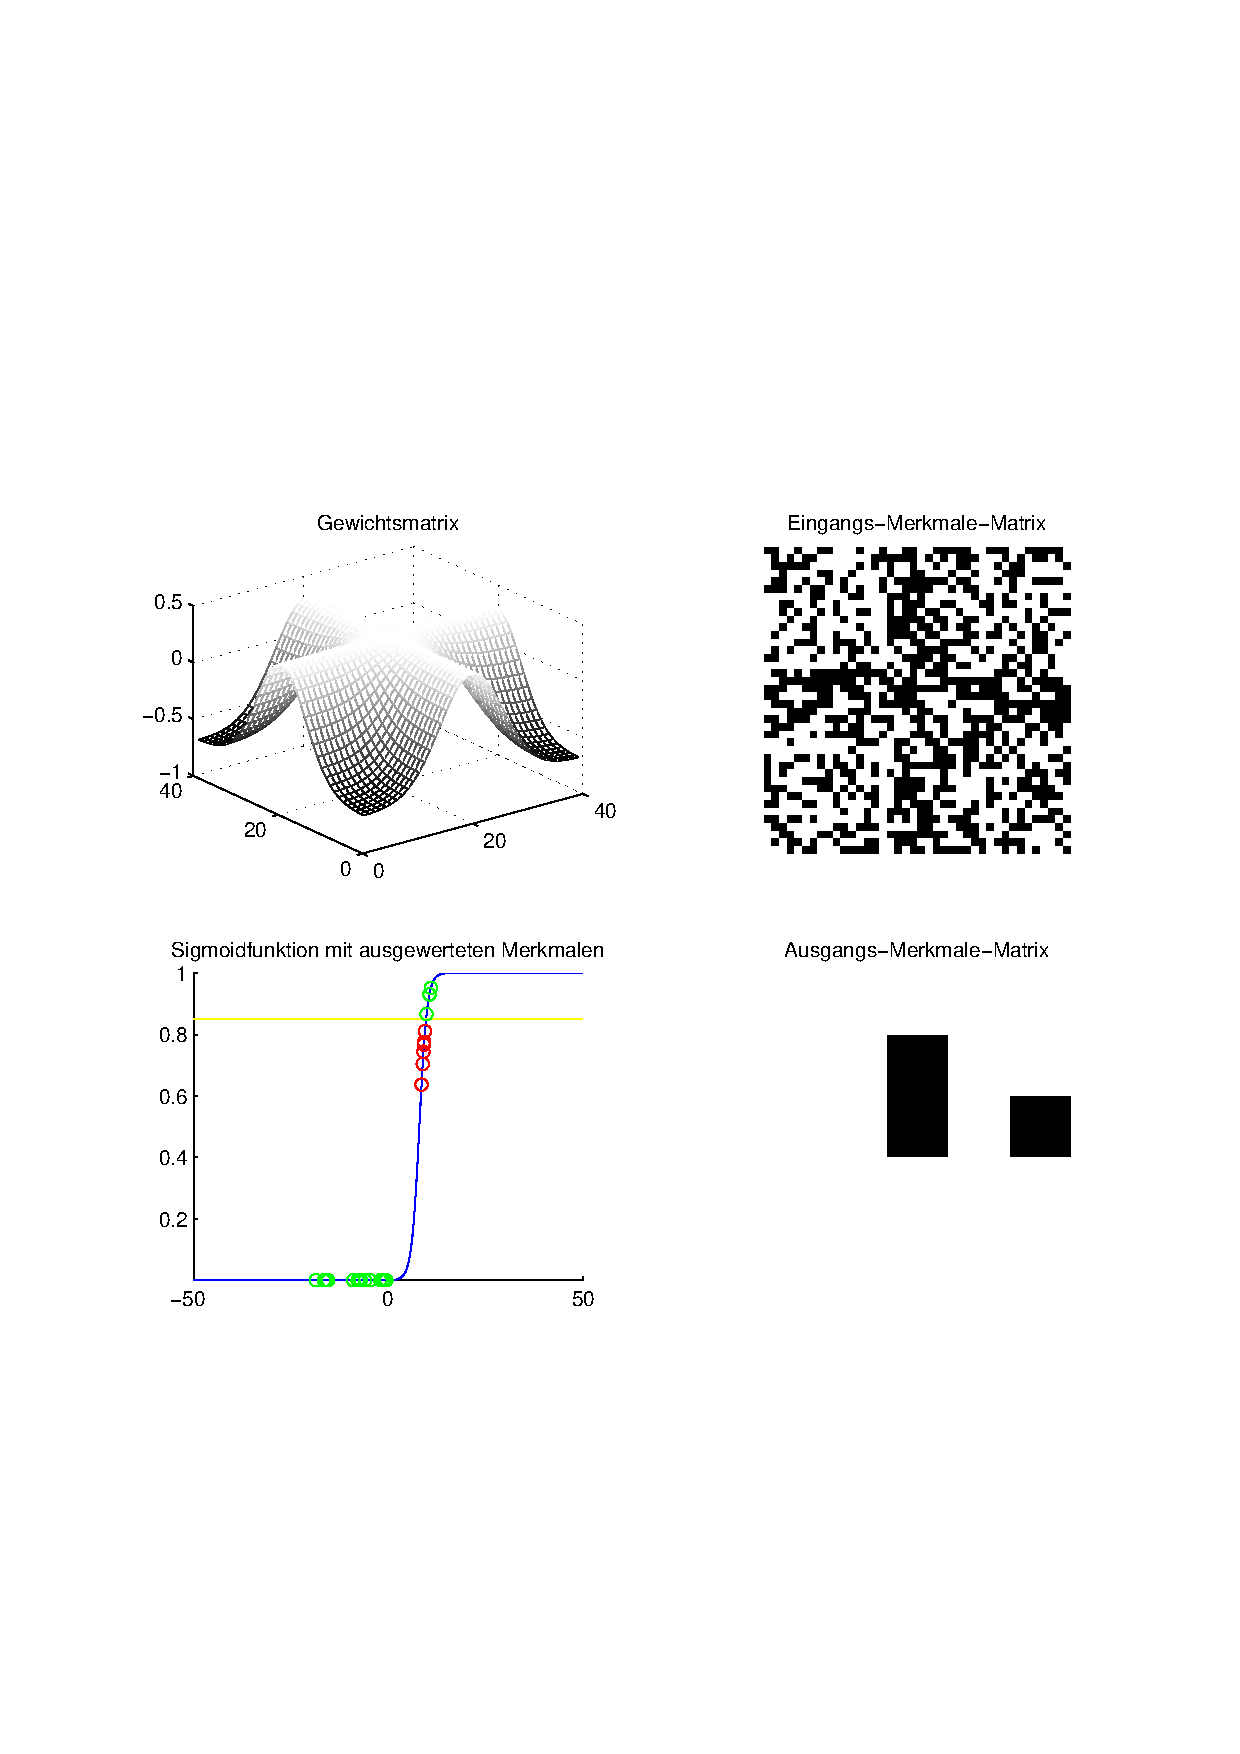
\includegraphics[width=\textwidth]{./Bilder/Auswertung/Endergebnis/TypeAddMul_Rauschen80_Cross_Layer1}
		\caption{AddMul, Kreuz, 80\% Rauschen, 1. Neuronen Ebene}
		\label{AddMul_Kreuz_80_1}
	\end{minipage}
	\vfill
	\begin{minipage}{0.8 \textwidth}
		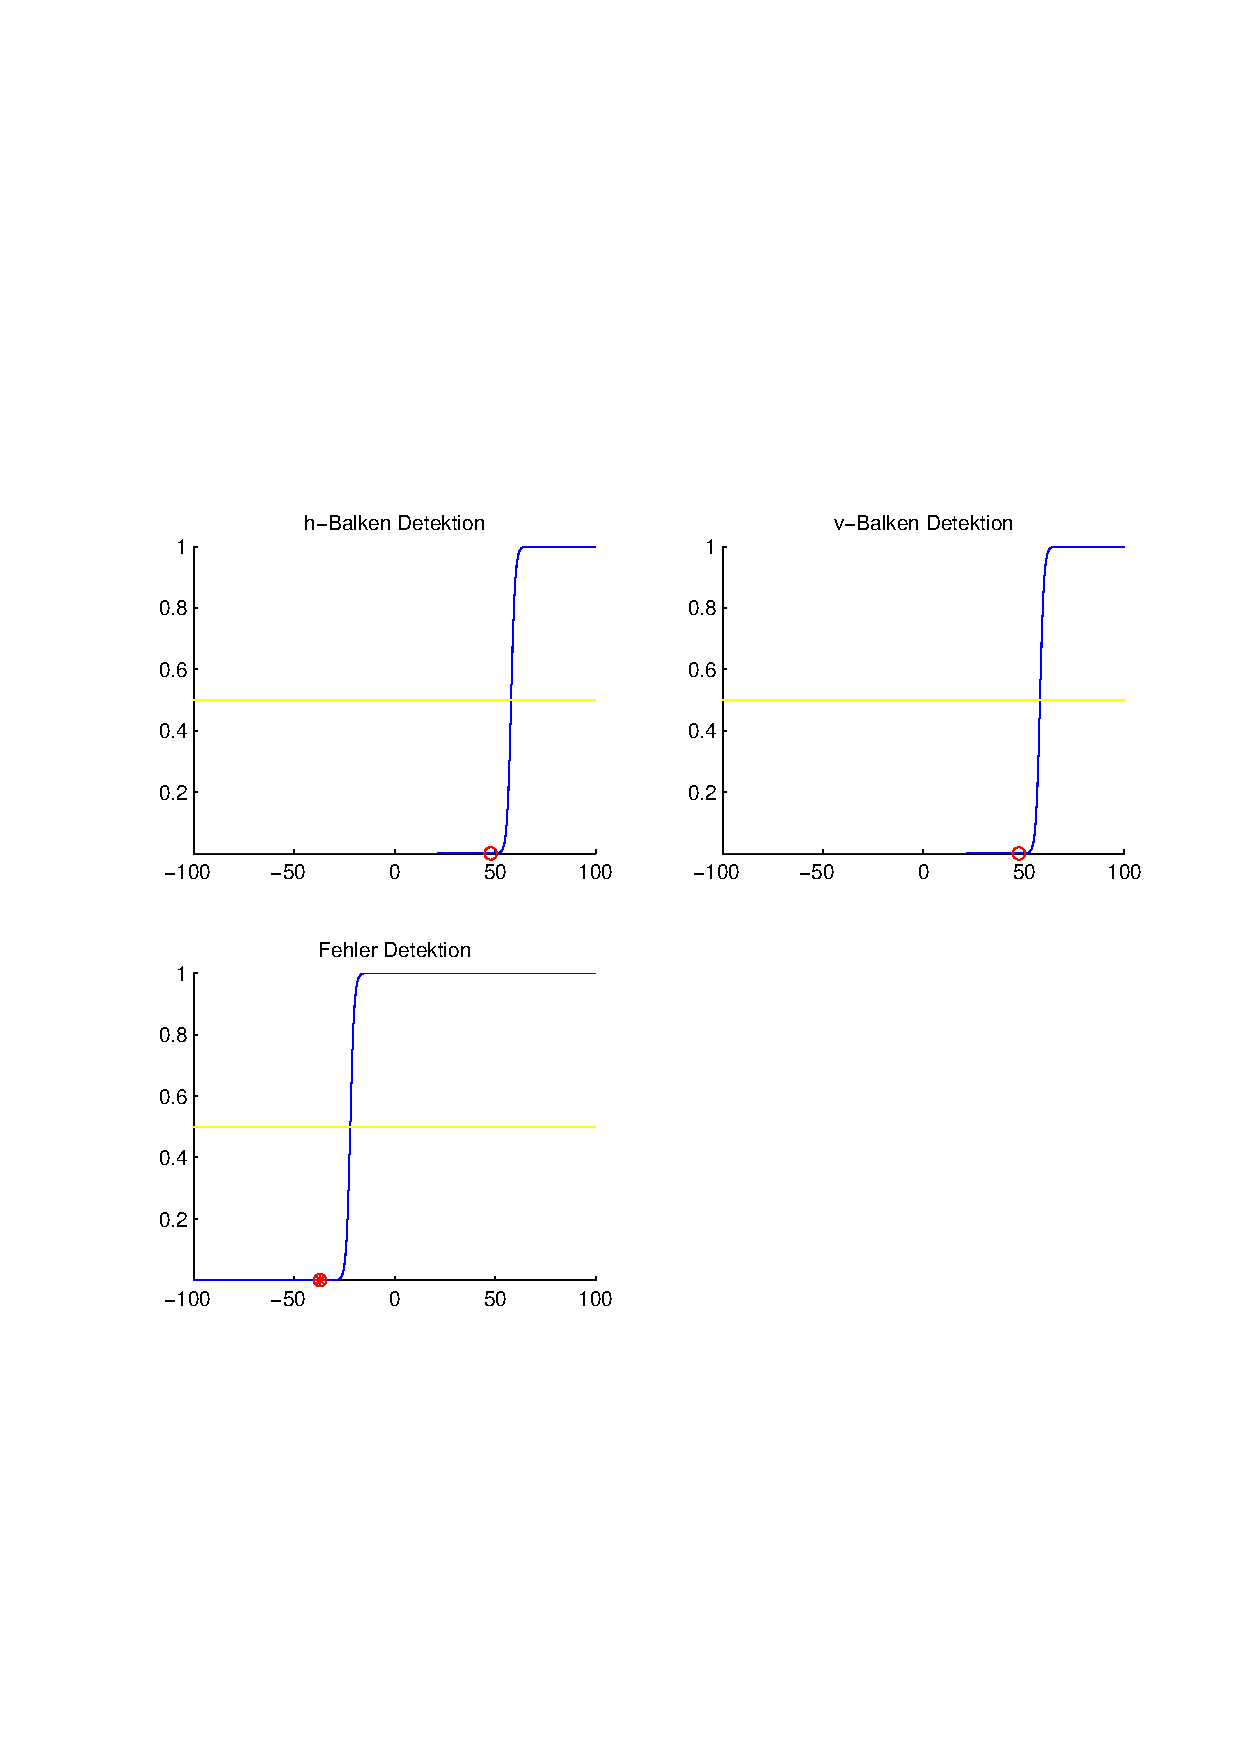
\includegraphics[width=\textwidth]{./Bilder/Auswertung/Endergebnis/TypeAddMul_Rauschen80_Cross_Layer2}
		\caption{AddMul, Kreuz, 80\% Rauschen, 2. Neuronen Ebene}
		\label{AddMul_Kreuz_80_2}
	\end{minipage}
\end{figure}
\clearpage

\subsection{Special Gewichtsmatrix}
\subsubsection{H-Balken}
\begin{figure}[hbt]
	\begin{minipage}{0.8 \textwidth}
		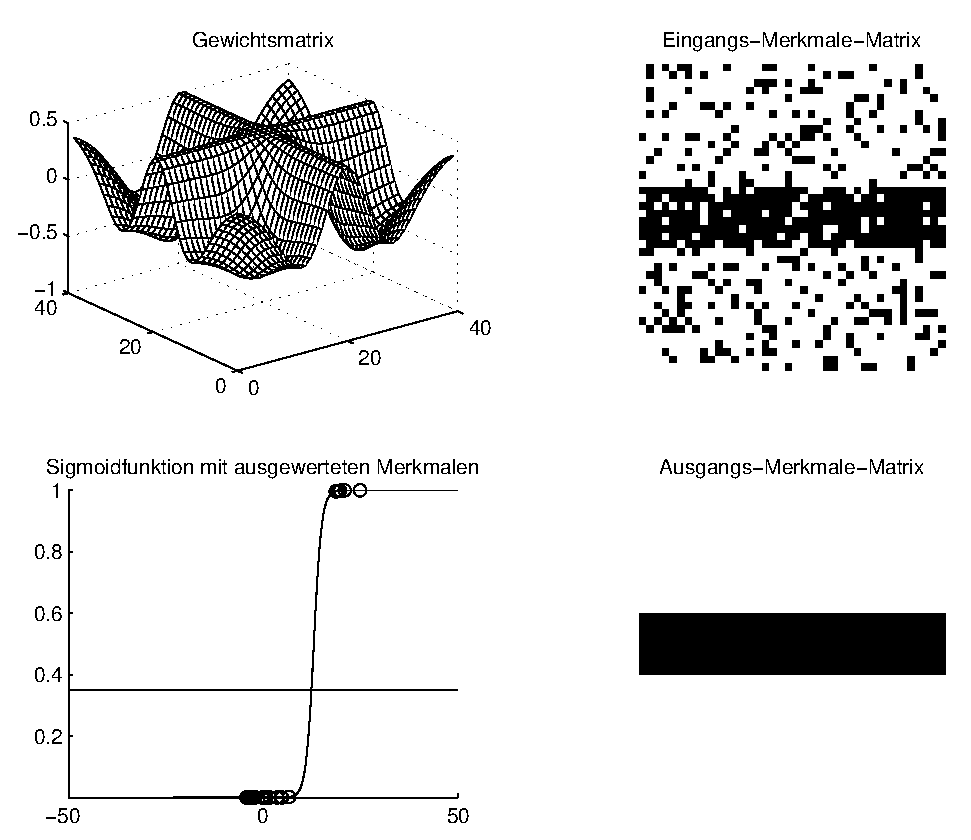
\includegraphics[width=\textwidth]{./Bilder/Auswertung/Endergebnis/TypeSpecial_Rauschen40_H_Line_Layer1}
		\caption{Special, H-Balken, 40\% Rauschen, 1. Neuronen Ebene}
		\label{Special_H_40_1}
	\end{minipage}
	\vfill
	\begin{minipage}{0.8 \textwidth}
		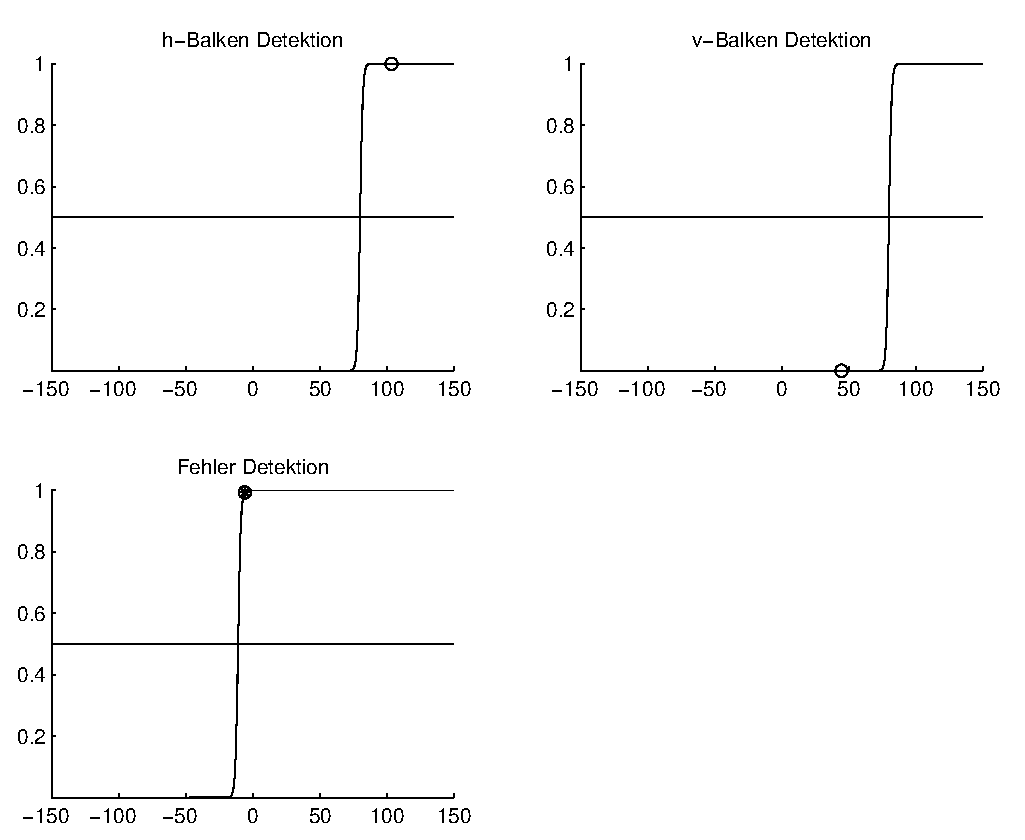
\includegraphics[width=\textwidth]{./Bilder/Auswertung/Endergebnis/TypeSpecial_Rauschen40_H_Line_Layer2}
		\caption{Special, H-Balken, 40\% Rauschen, 2. Neuronen Ebene}
		\label{Special_H_40_2}
	\end{minipage}
\end{figure}

\begin{figure}[hbt]
	\begin{minipage}{0.8 \textwidth}
		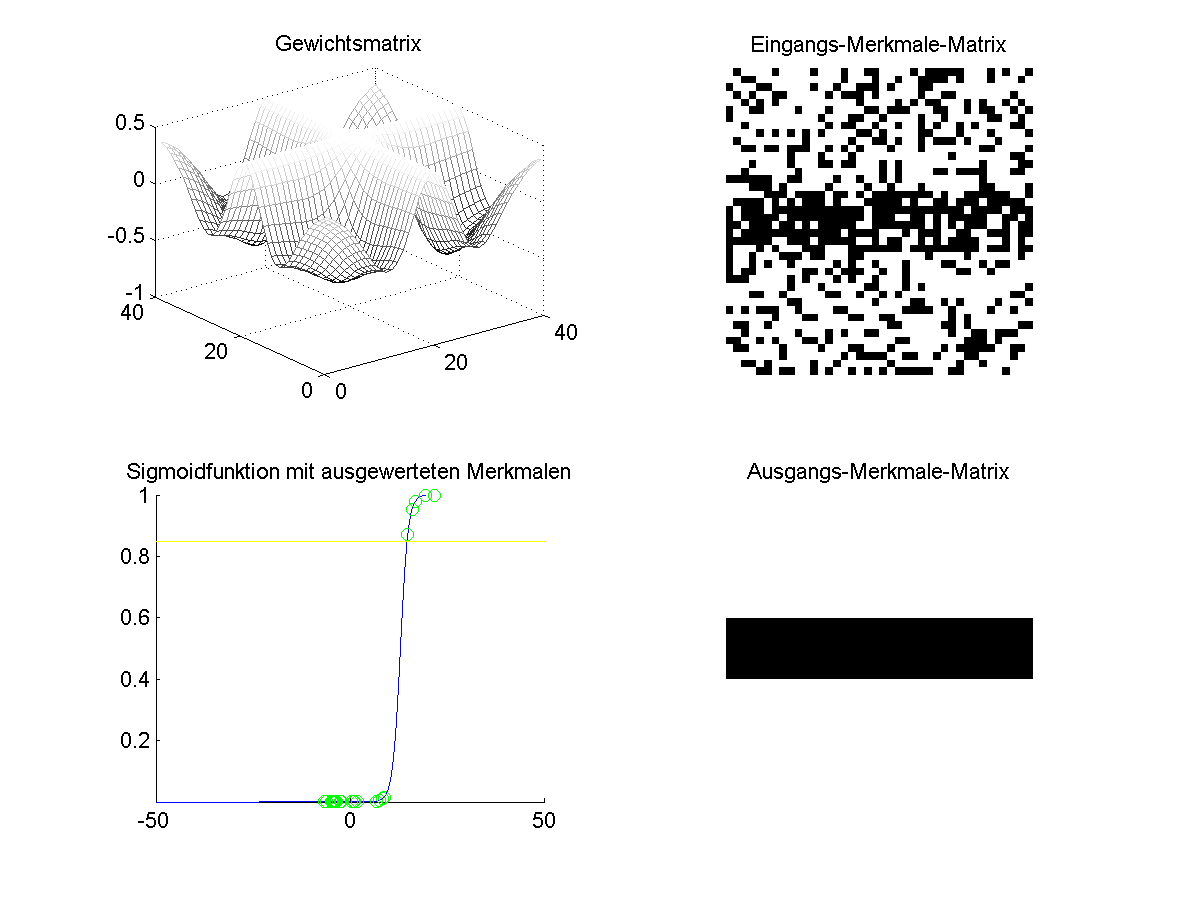
\includegraphics[width=\textwidth]{./Bilder/Auswertung/Endergebnis/TypeSpecial_Rauschen60_H_Line_Layer1}
		\caption{Special, H-Balken, 60\% Rauschen, 1. Neuronen Ebene}
		\label{Special_H_60_1}
	\end{minipage}
	\vfill
	\begin{minipage}{0.8 \textwidth}
		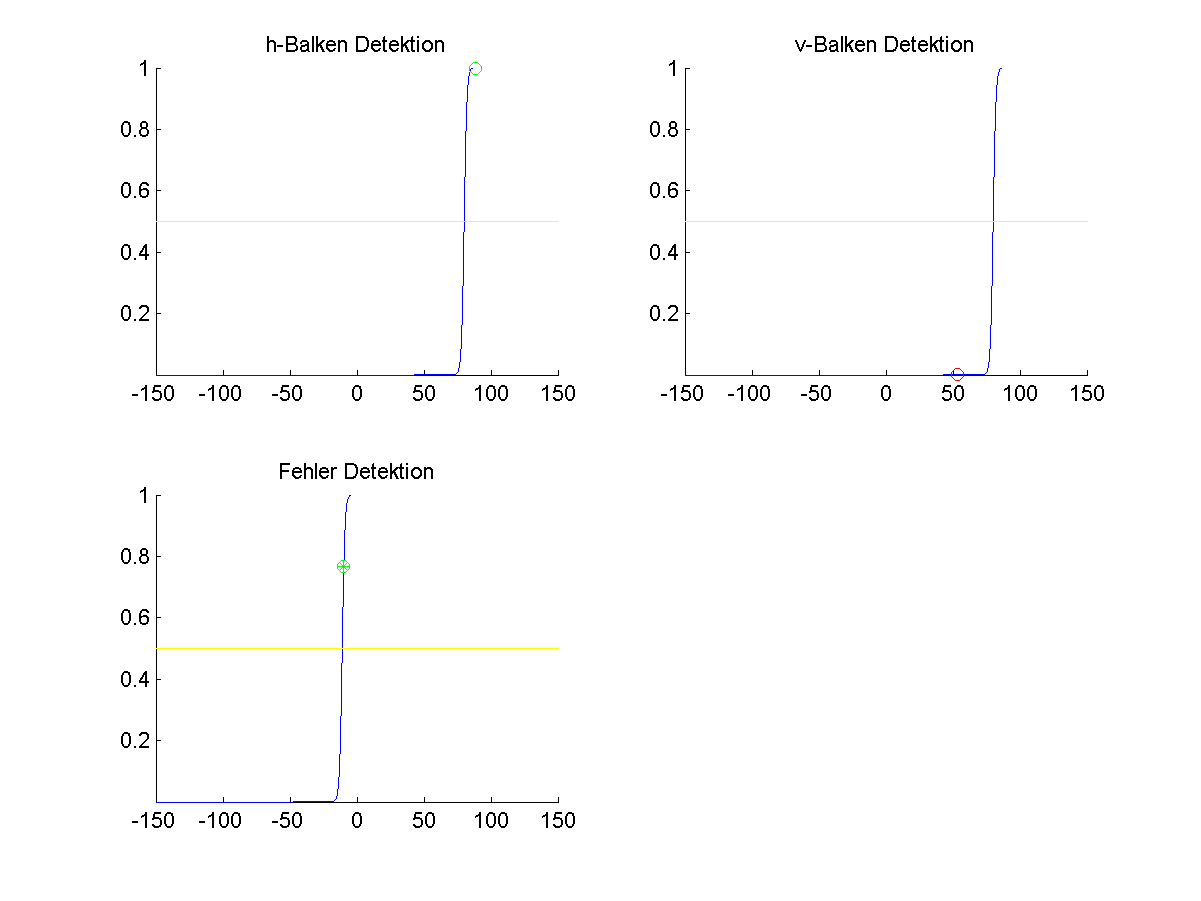
\includegraphics[width=\textwidth]{./Bilder/Auswertung/Endergebnis/TypeSpecial_Rauschen60_H_Line_Layer2}
		\caption{Special, H-Balken, 60\% Rauschen, 2. Neuronen Ebene}
		\label{Special_H_60_2}
	\end{minipage}
\end{figure}

\begin{figure}[hbt]
	\begin{minipage}{0.8 \textwidth}
		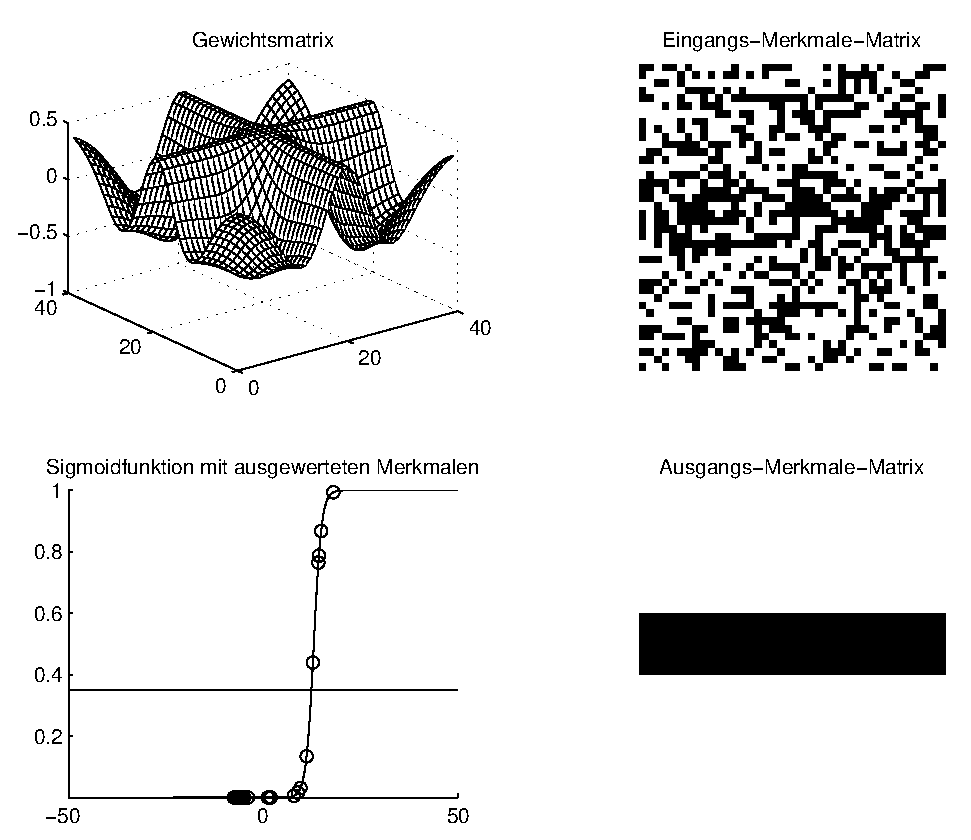
\includegraphics[width=\textwidth]{./Bilder/Auswertung/Endergebnis/TypeSpecial_Rauschen80_H_Line_Layer1}
		\caption{Special, H-Balken, 80\% Rauschen, 1. Neuronen Ebene}
		\label{Special_H_80_1}
	\end{minipage}
	\vfill
	\begin{minipage}{0.8 \textwidth}
		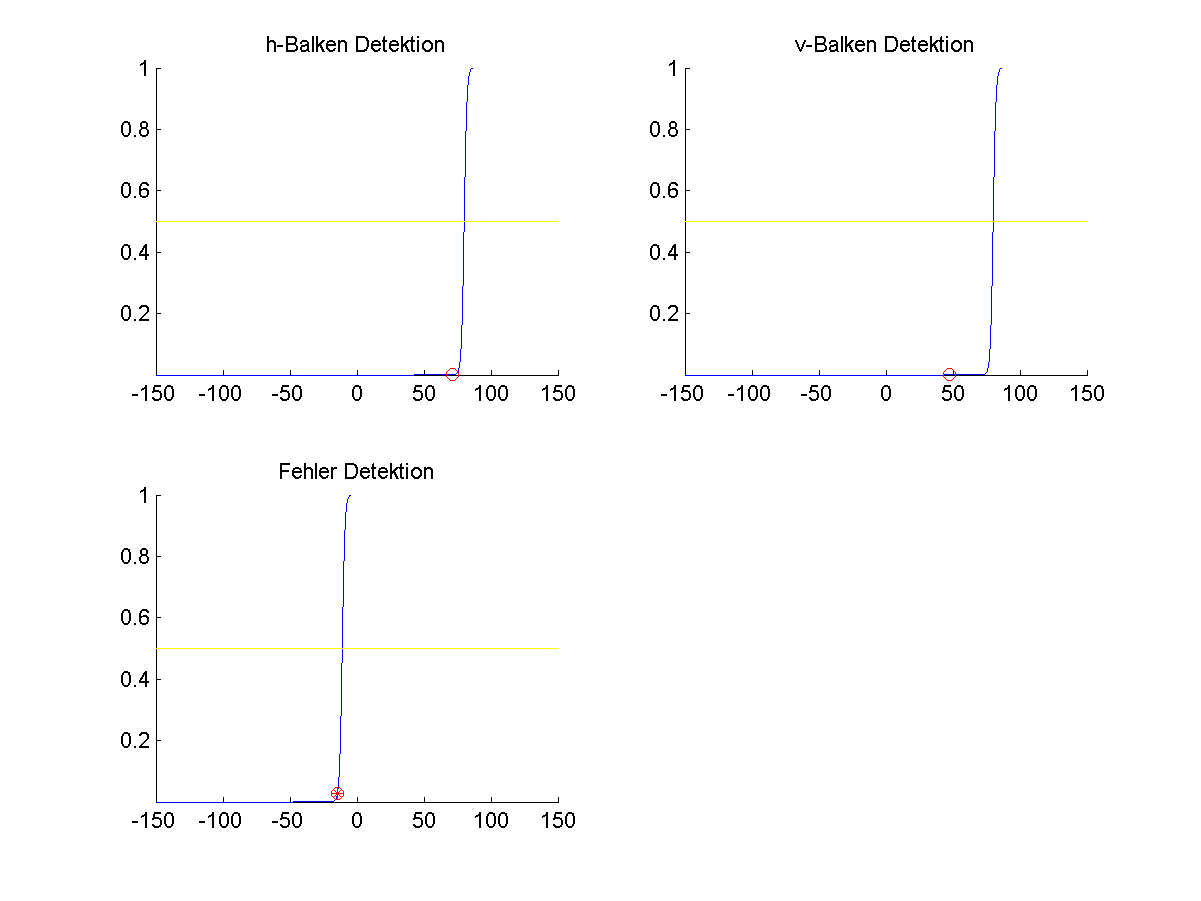
\includegraphics[width=\textwidth]{./Bilder/Auswertung/Endergebnis/TypeSpecial_Rauschen80_H_Line_Layer2}
		\caption{Special, H-Balken, 80\% Rauschen, 2. Neuronen Ebene}
		\label{Special_H_80_2}
	\end{minipage}
\end{figure}
\clearpage

\subsubsection{V-Balken}
\begin{figure}[hbt]
	\begin{minipage}{0.8 \textwidth}
		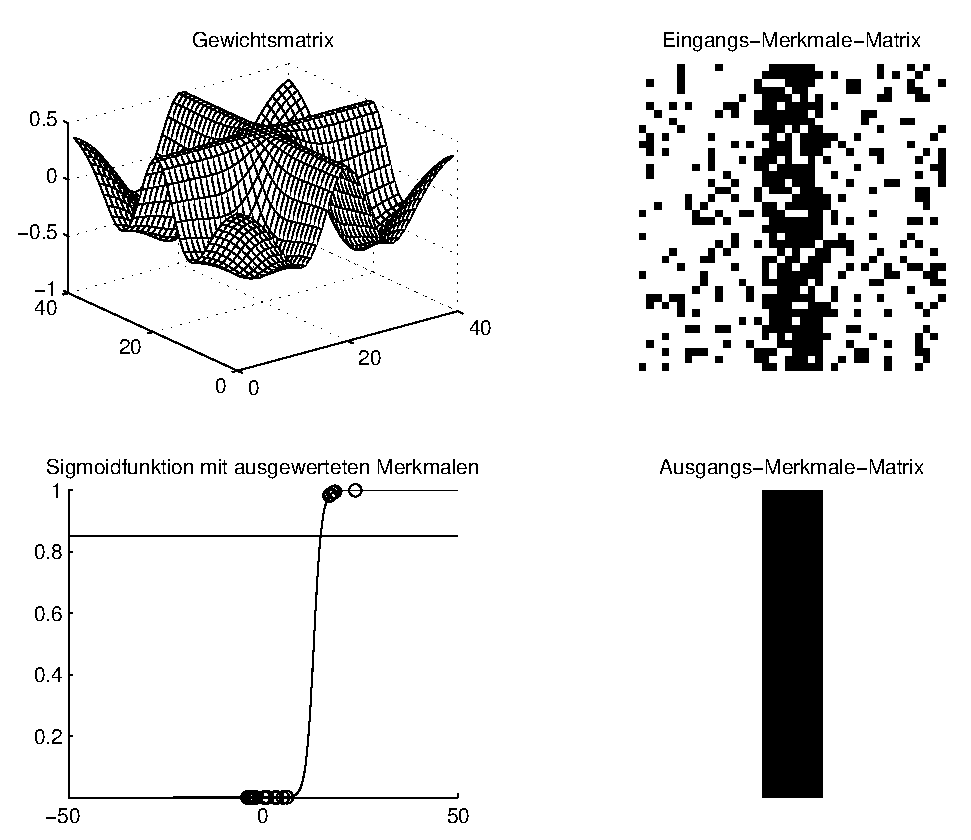
\includegraphics[width=\textwidth]{./Bilder/Auswertung/Endergebnis/TypeSpecial_Rauschen40_V_Line_Layer1}
		\caption{Special, V-Balken, 40\% Rauschen, 1. Neuronen Ebene}
		\label{Special_V_40_1}
	\end{minipage}
	\vfill
	\begin{minipage}{0.8 \textwidth}
		\includegraphics[width=\textwidth]{./Bilder/Auswertung/Endergebnis/TypeSpecial_Rauschen40_v_Line_Layer2}
		\caption{Special, V-Balken, 40\% Rauschen, 2. Neuronen Ebene}
		\label{Special_V_40_2}
	\end{minipage}
\end{figure}

\begin{figure}[hbt]
	\begin{minipage}{0.8 \textwidth}
		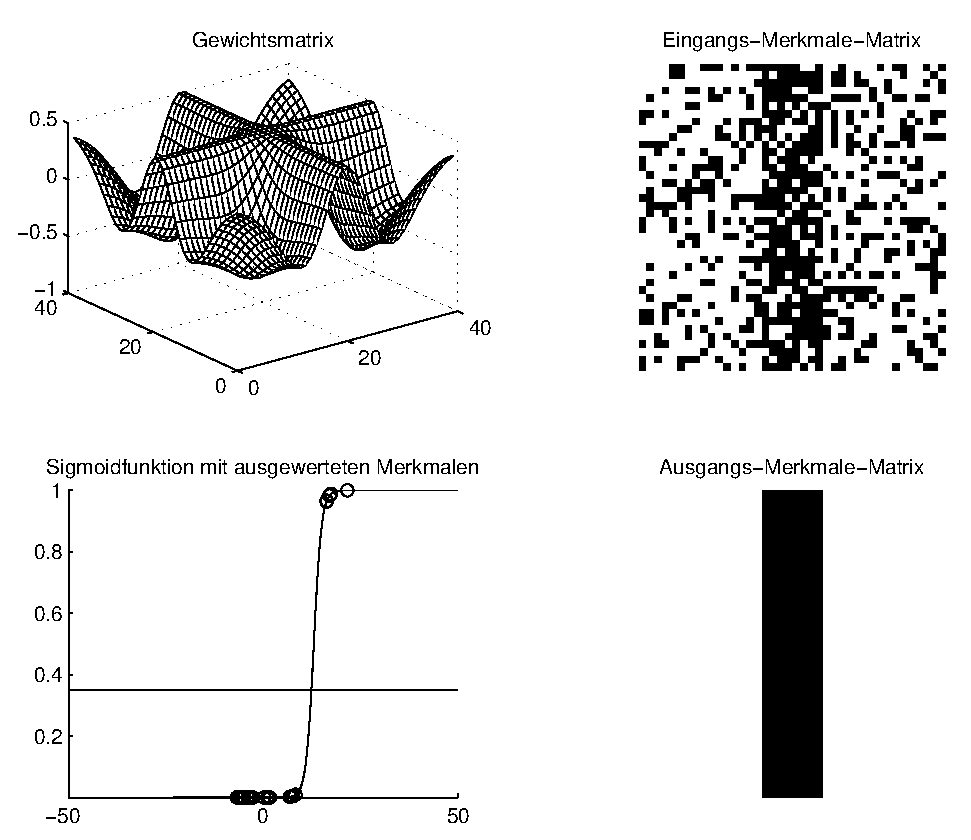
\includegraphics[width=\textwidth]{./Bilder/Auswertung/Endergebnis/TypeSpecial_Rauschen60_V_Line_Layer1}
		\caption{Special, V-Balken, 60\% Rauschen, 1. Neuronen Ebene}
		\label{Special_V_60_1}
	\end{minipage}
	\vfill
	\begin{minipage}{0.8 \textwidth}
		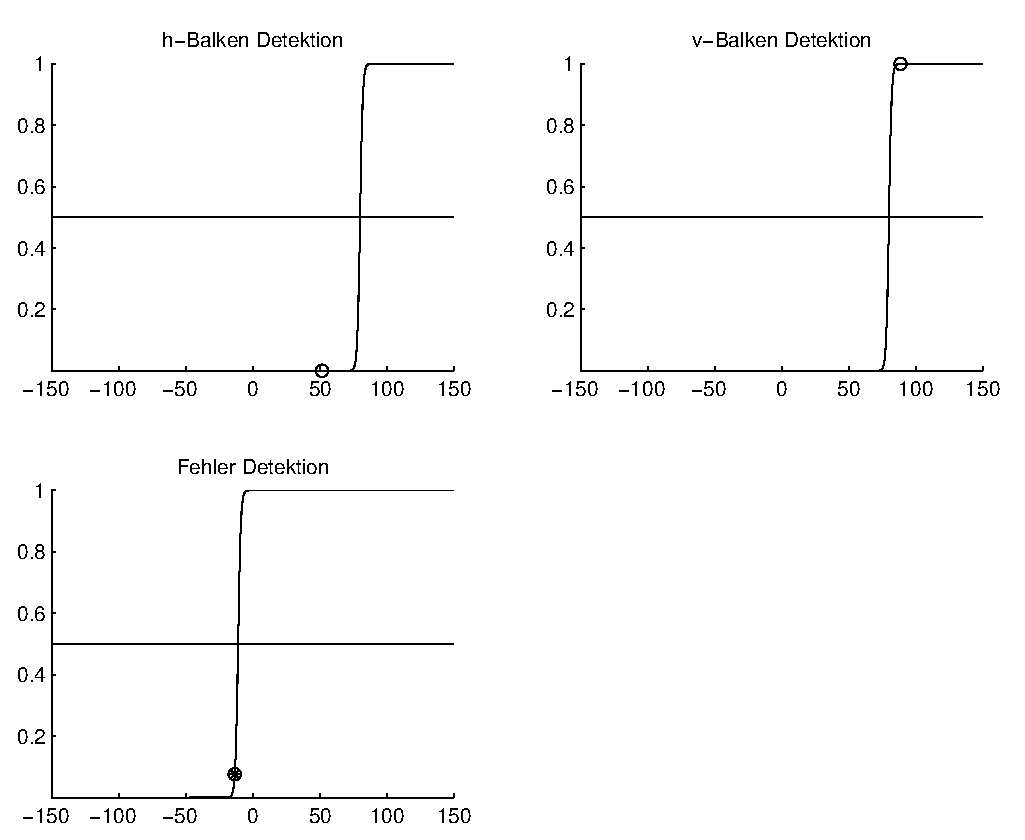
\includegraphics[width=\textwidth]{./Bilder/Auswertung/Endergebnis/TypeSpecial_Rauschen60_V_Line_Layer2}
		\caption{Special, V-Balken, 60\% Rauschen, 2. Neuronen Ebene}
		\label{Special_V_60_2}
	\end{minipage}
\end{figure}

\begin{figure}[hbt]
	\begin{minipage}{0.8 \textwidth}
		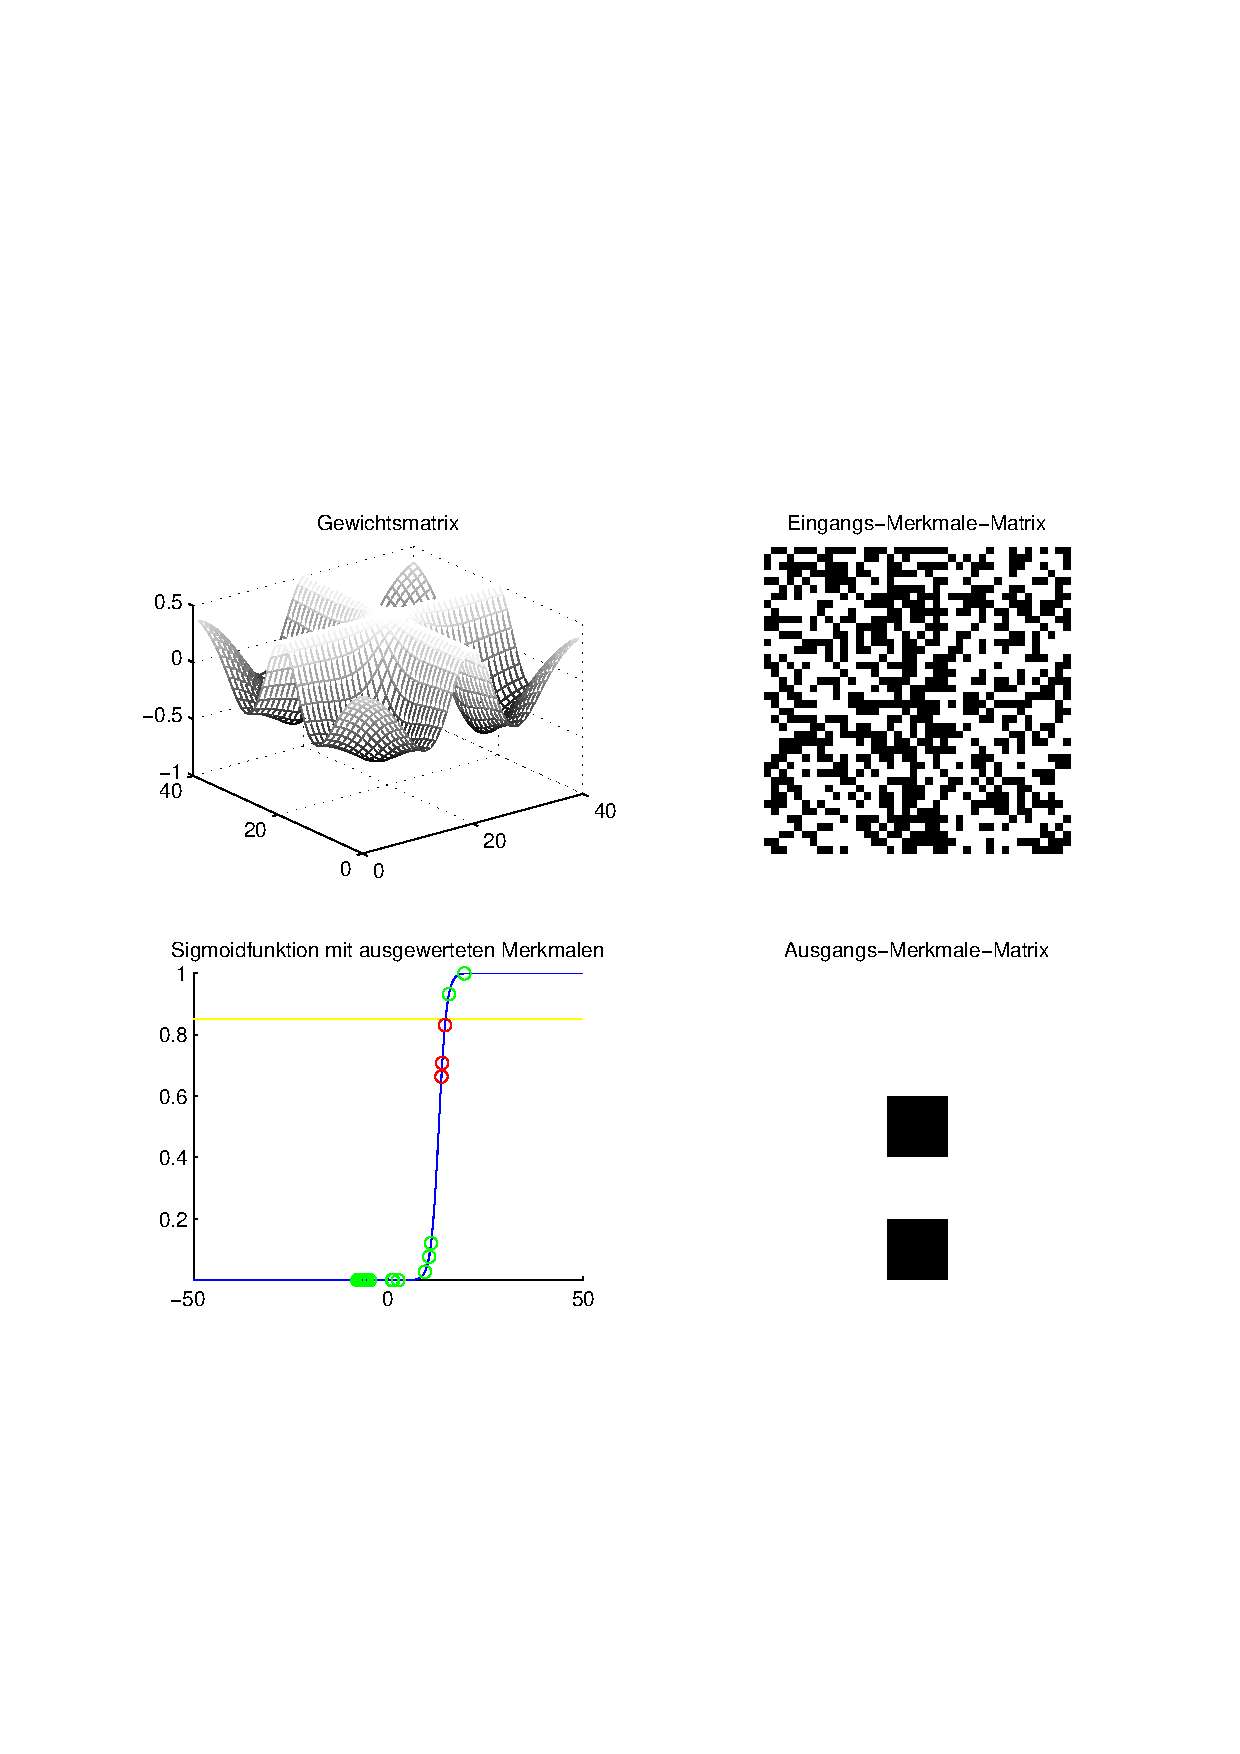
\includegraphics[width=\textwidth]{./Bilder/Auswertung/Endergebnis/TypeSpecial_Rauschen80_V_Line_Layer1}
		\caption{Special, V-Balken, 80\% Rauschen, 1. Neuronen Ebene}
		\label{Special_V_80_1}
	\end{minipage}
	\vfill
	\begin{minipage}{0.8 \textwidth}
		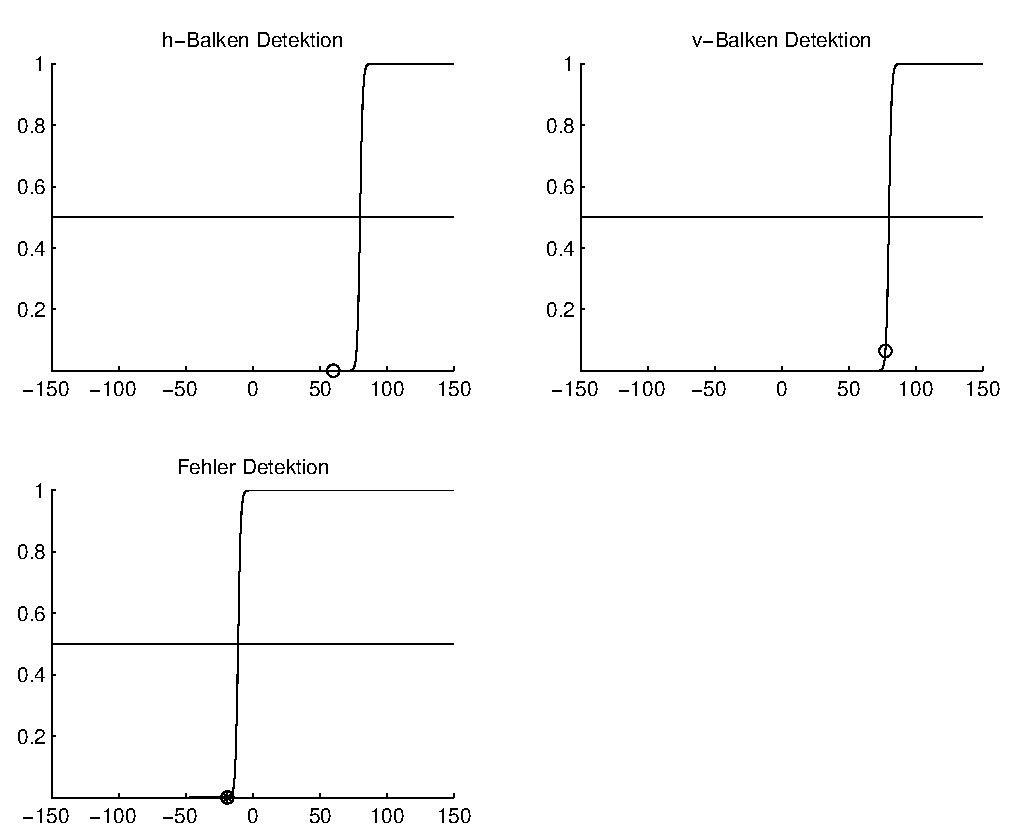
\includegraphics[width=\textwidth]{./Bilder/Auswertung/Endergebnis/TypeSpecial_Rauschen80_V_Line_Layer2}
		\caption{Special, V-Balken, 80\% Rauschen, 2. Neuronen Ebene}
		\label{Special_V_80_2}
	\end{minipage}
\end{figure}
\clearpage

\subsubsection{Kreuz}
\begin{figure}[hbt]
	\begin{minipage}{0.8 \textwidth}
		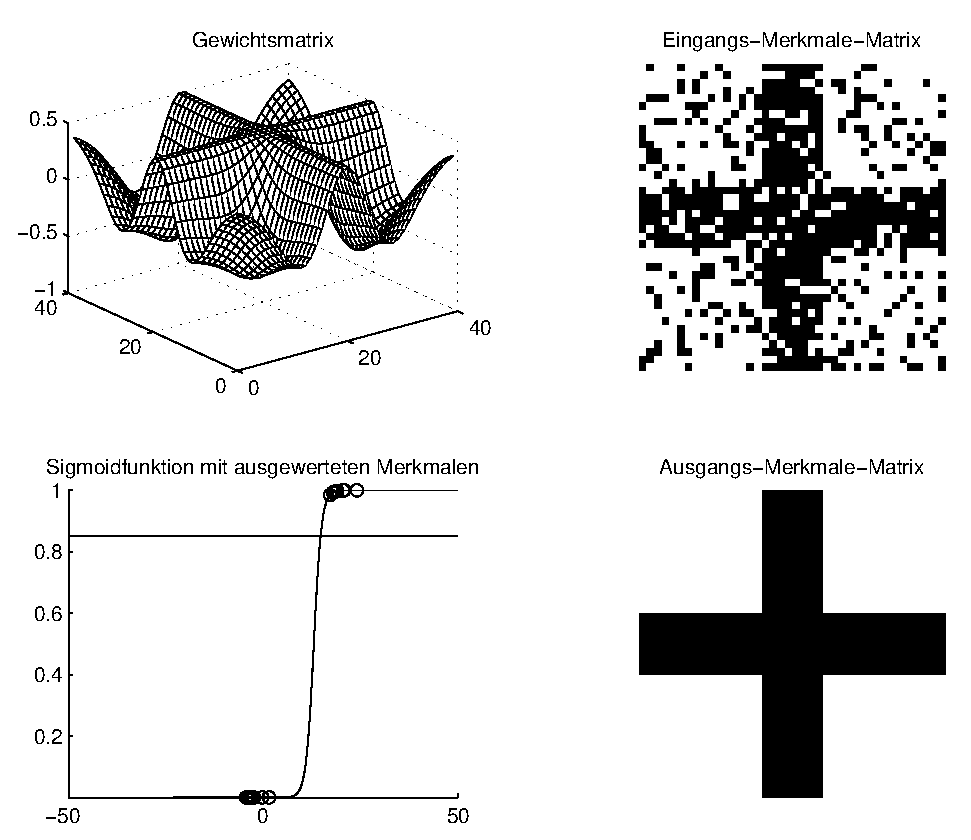
\includegraphics[width=\textwidth]{./Bilder/Auswertung/Endergebnis/TypeSpecial_Rauschen40_Cross_Layer1}
		\caption{Special, Kreuz, 40\% Rauschen, 1. Neuronen Ebene}
		\label{Special_Kreuz_40_1}
	\end{minipage}
	\vfill
	\begin{minipage}{0.8 \textwidth}
		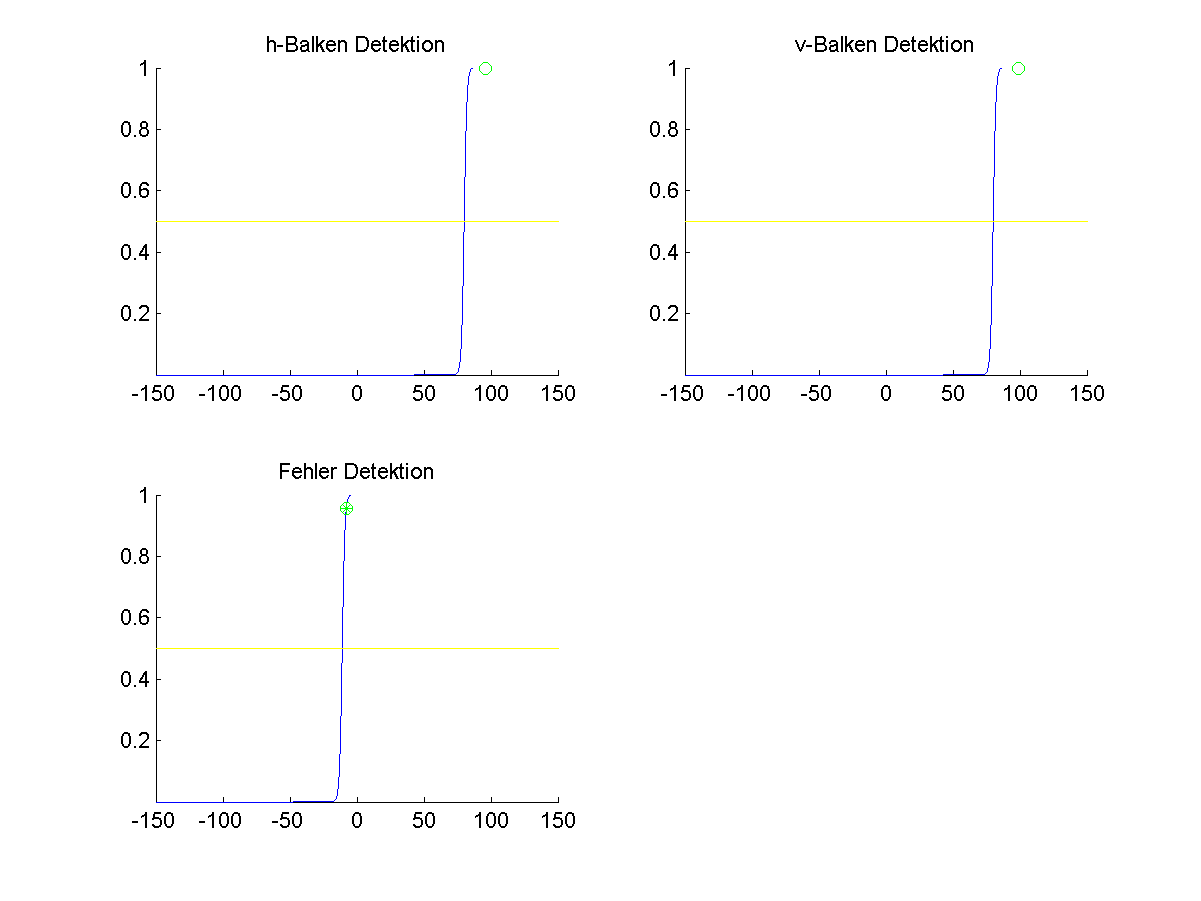
\includegraphics[width=\textwidth]{./Bilder/Auswertung/Endergebnis/TypeSpecial_Rauschen40_Cross_Layer2}
		\caption{Special, Kreuz, 40\% Rauschen, 2. Neuronen Ebene}
		\label{Special_Kreuz_40_2}
	\end{minipage}
\end{figure}

\begin{figure}[hbt]
	\begin{minipage}{0.8 \textwidth}
		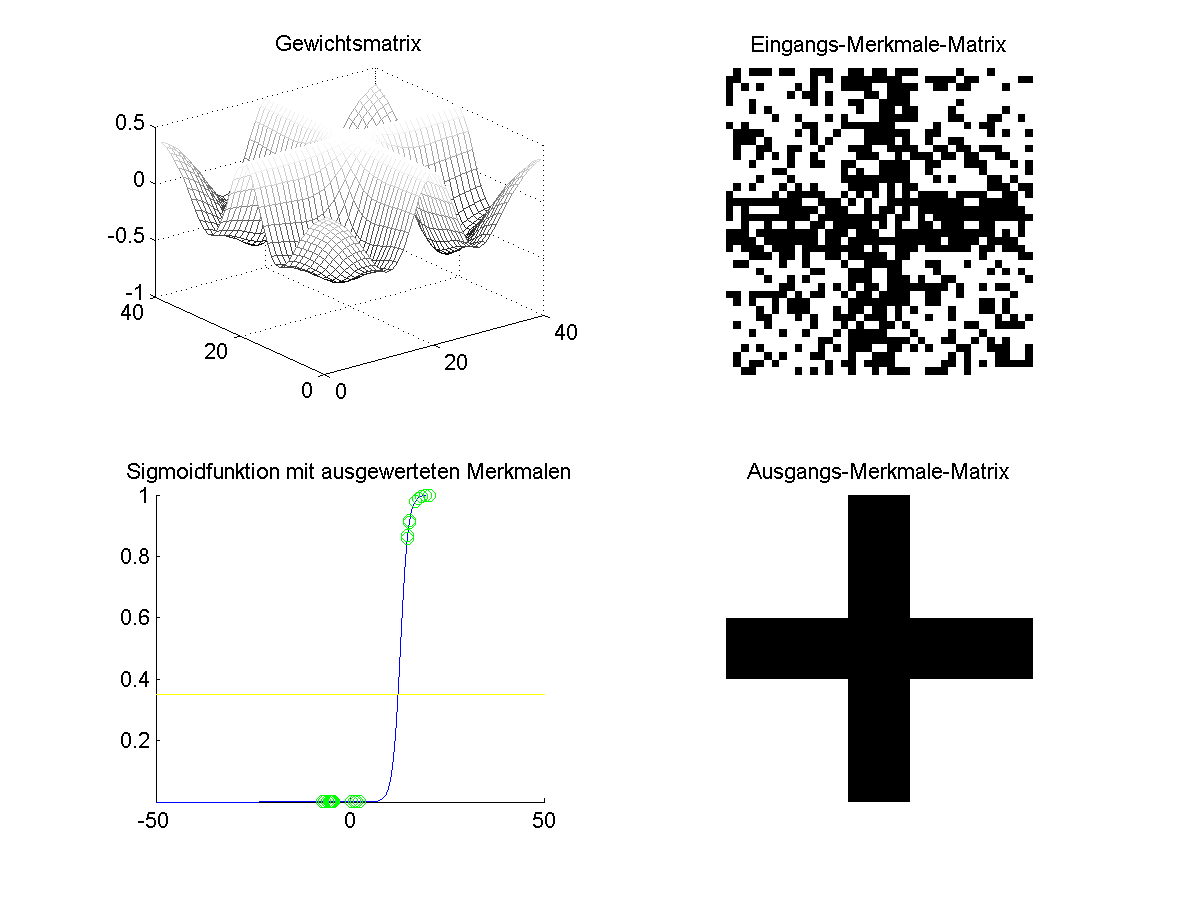
\includegraphics[width=\textwidth]{./Bilder/Auswertung/Endergebnis/TypeSpecial_Rauschen60_Cross_Layer1}
		\caption{Special, Kreuz, 60\% Rauschen, 1. Neuronen Ebene}
		\label{Special_Kreuz_60_1}
	\end{minipage}
	\vfill
	\begin{minipage}{0.8 \textwidth}
		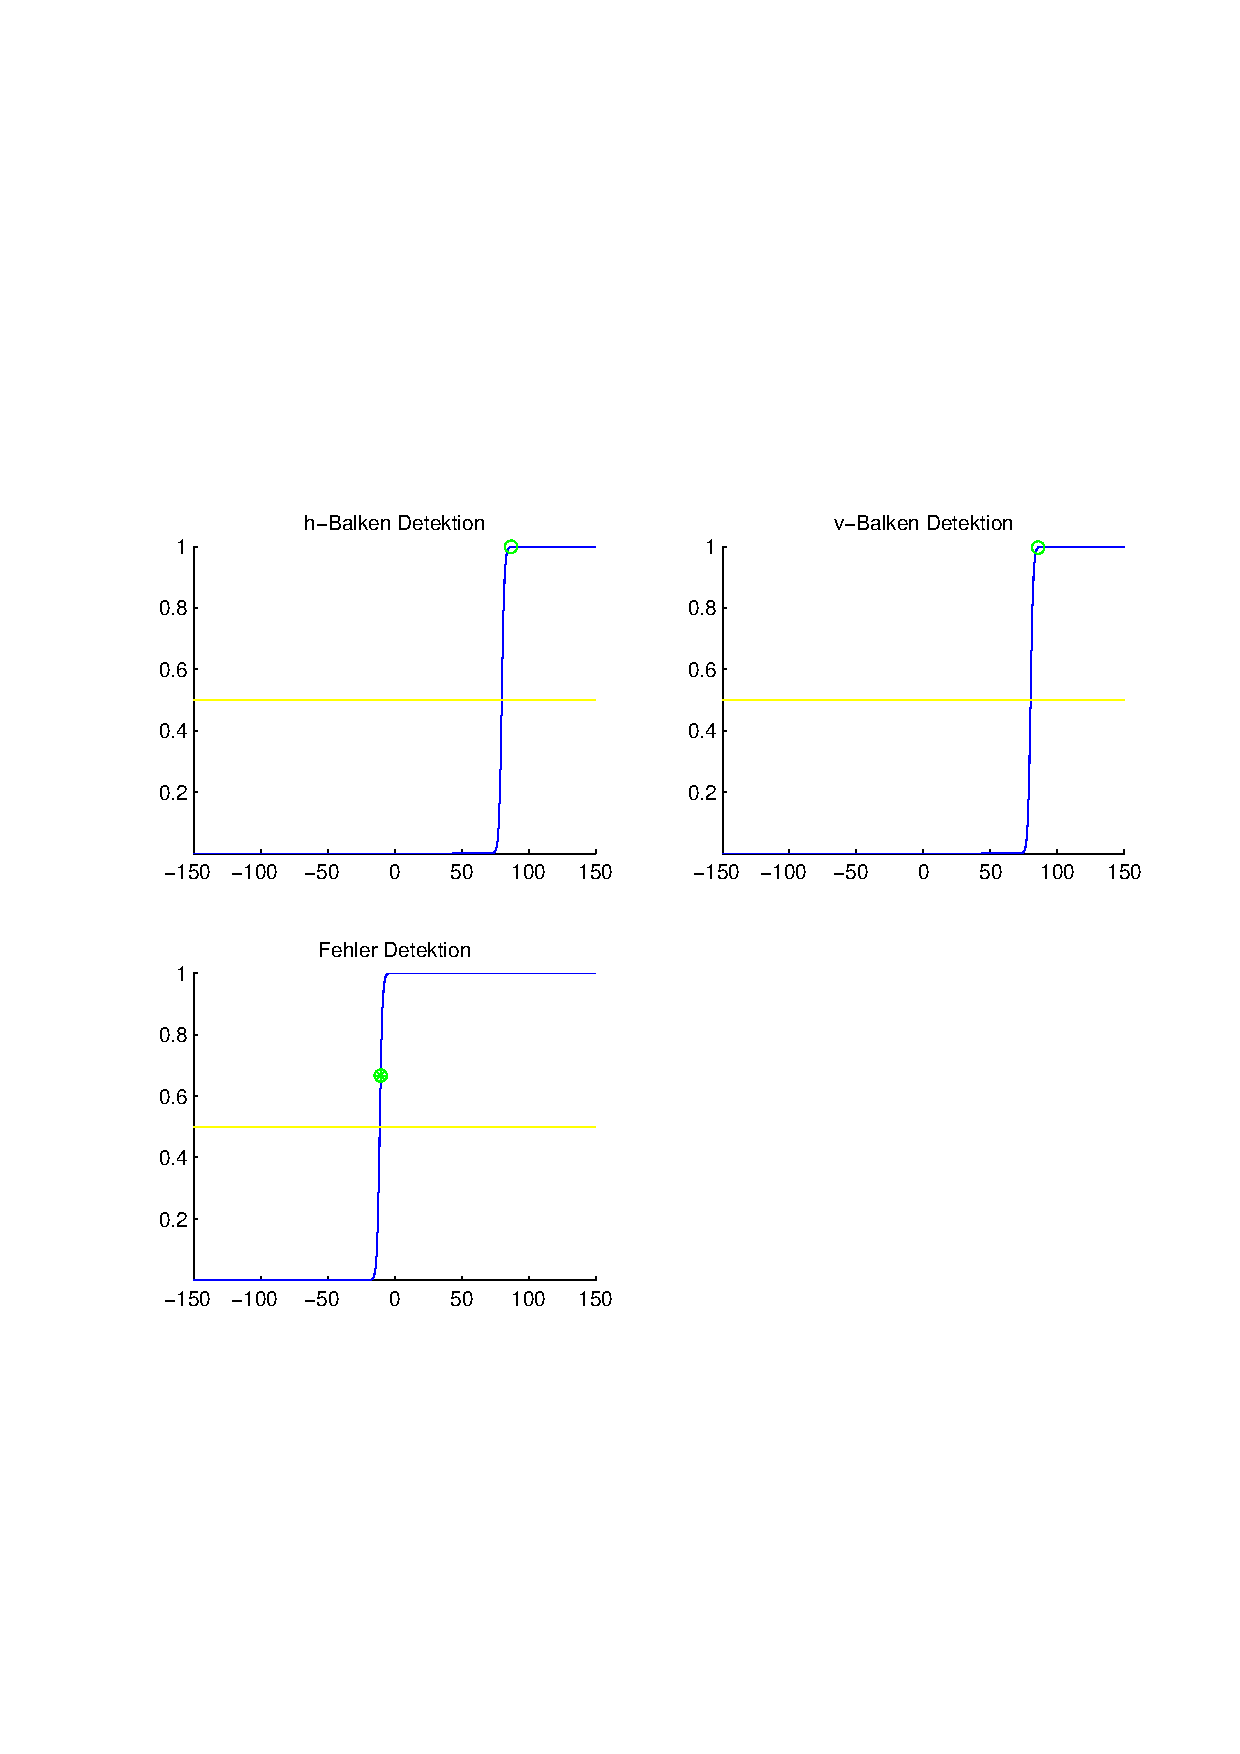
\includegraphics[width=\textwidth]{./Bilder/Auswertung/Endergebnis/TypeSpecial_Rauschen60_Cross_Layer2}
		\caption{Special, Kreuz, 60\% Rauschen, 2. Neuronen Ebene}
		\label{Special_Kreuz_60_2}
	\end{minipage}
\end{figure}

\begin{figure}[hbt]
	\begin{minipage}{0.8 \textwidth}
		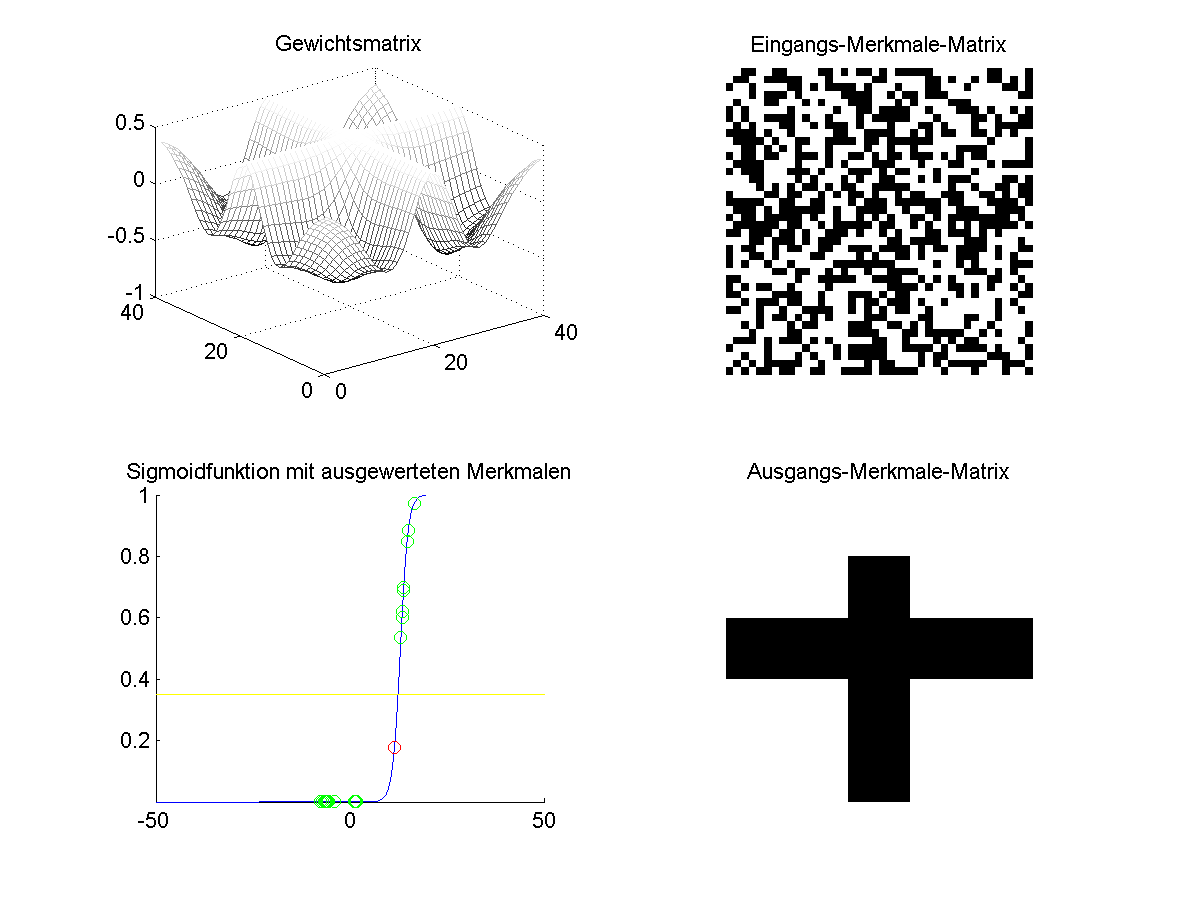
\includegraphics[width=\textwidth]{./Bilder/Auswertung/Endergebnis/TypeSpecial_Rauschen80_Cross_Layer1}
		\caption{Special, Kreuz, 80\% Rauschen, 1. Neuronen Ebene}
		\label{Special_Kreuz_80_1}
	\end{minipage}
	\vfill
	\begin{minipage}{0.8 \textwidth}
		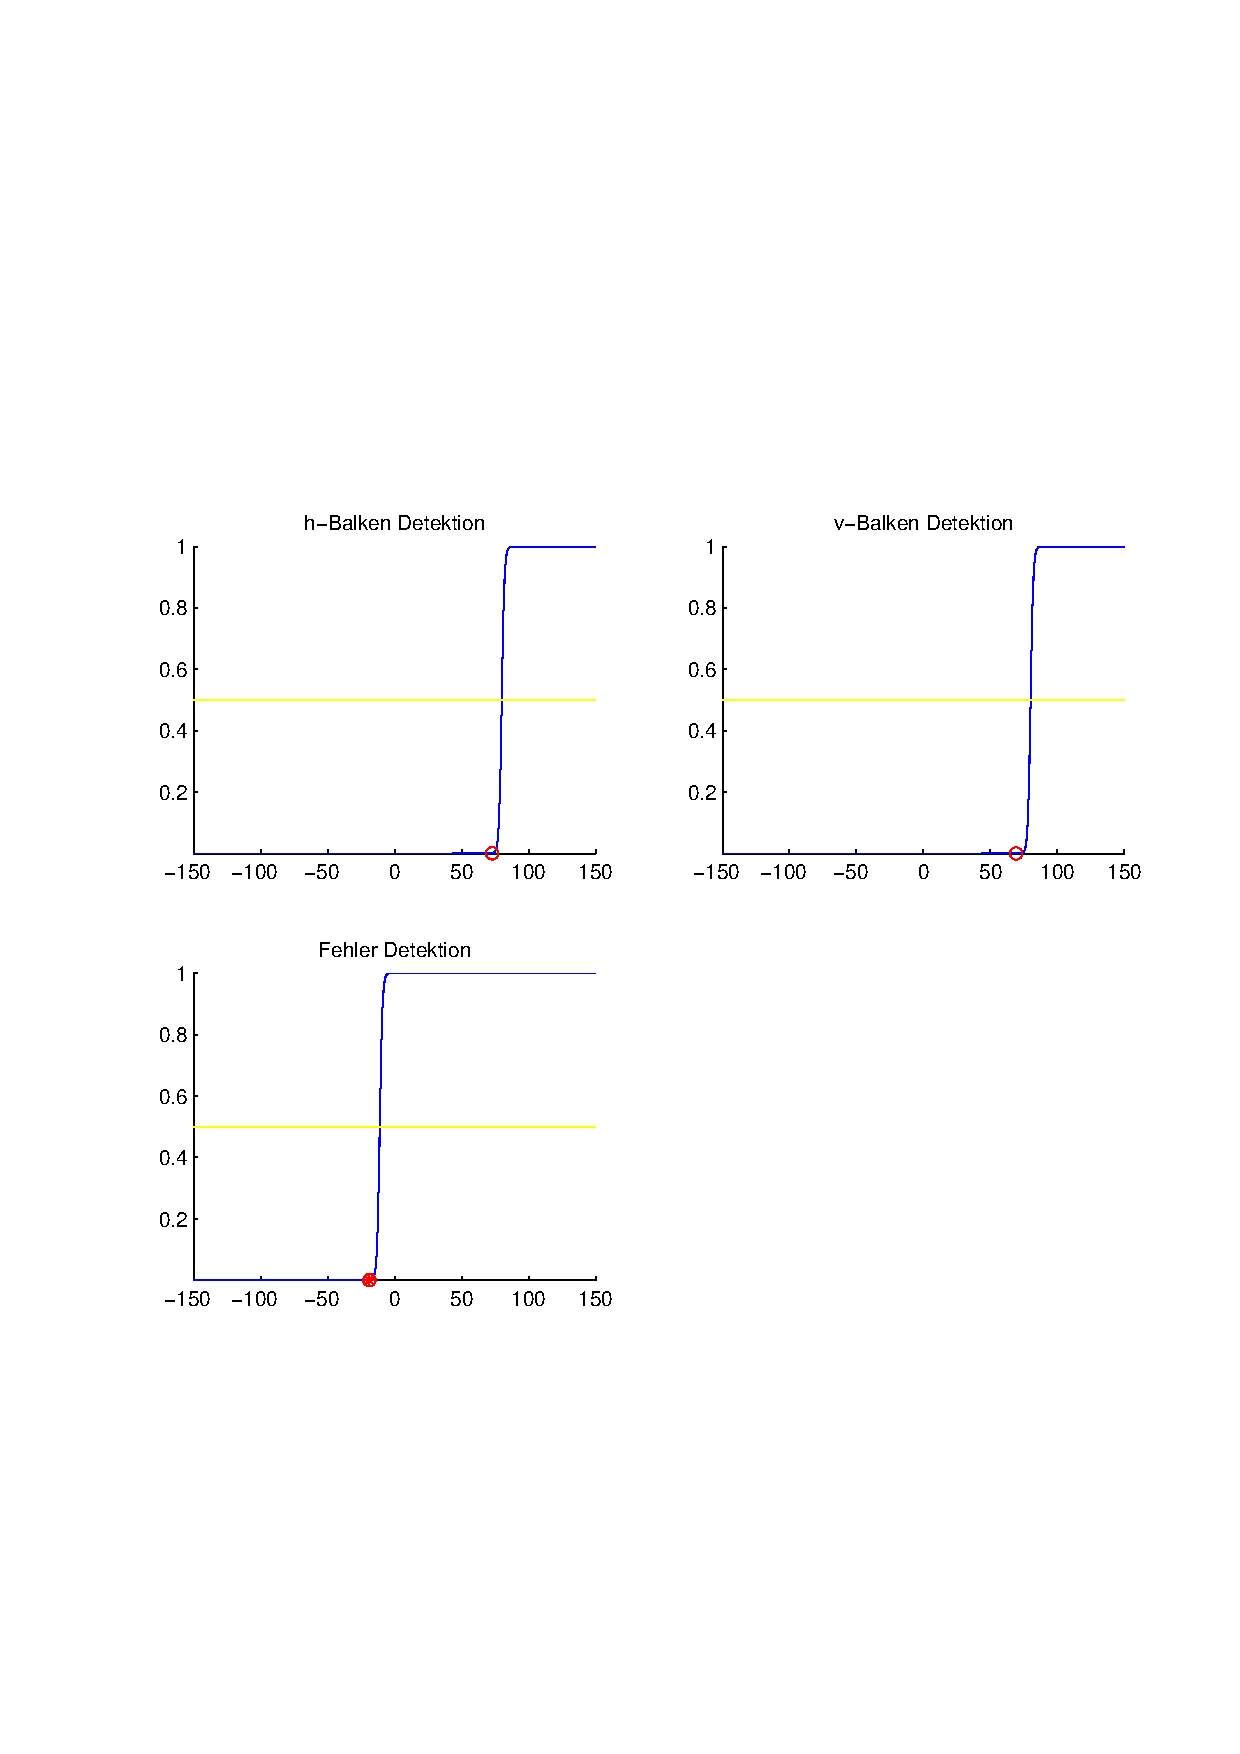
\includegraphics[width=\textwidth]{./Bilder/Auswertung/Endergebnis/TypeSpecial_Rauschen80_Cross_Layer2}
		\caption{Special, Kreuz, 80\% Rauschen, 2. Neuronen Ebene}
		\label{Special_Kreuz_80_2}
	\end{minipage}
\end{figure}
\clearpage

